% Artículo IEEE Transactions on AI
% Taller de RAG - Procesamiento de Lenguaje Natural
% Pontificia Universidad Javeriana, Maestría en Inteligencia Artificial

\documentclass[journal]{IEEEtran}

\usepackage[spanish,es-nodecimaldot,es-noquoting]{babel}
\usepackage[T1]{fontenc}
\usepackage[utf8]{inputenc}
\usepackage{amsmath,amssymb}
\usepackage{graphicx}
\usepackage{booktabs}
\usepackage{multirow}
\usepackage{array}
\usepackage{url}
\usepackage{tikz}
\usetikzlibrary{arrows.meta,positioning,shapes.geometric}

\graphicspath{{../figuras/}{figuras/}}

\addto\captionsspanish{\renewcommand{\tablename}{Tabla}\renewcommand{\figurename}{Figura}}

\begin{document}

\title{Asistente RAG reproducible sobre prensa y Bluesky con Milvus y modelos locales: arquitectura, evaluaci\'on y compuerta de dominio}

\author{
\IEEEauthorblockN{Erika Valeria Rivera Jimenez}
\IEEEauthorblockA{Pontificia Universidad Javeriana\\
Bogot\'a, Colombia\\
riveraev@javeriana.edu.co}
\and
\IEEEauthorblockN{Julian Guillermo Carrillo Meneses}
\IEEEauthorblockA{Pontificia Universidad Javeriana\\
Bogot\'a, Colombia\\
carrillojuliang@javeriana.edu.co}
\and
\IEEEauthorblockN{Carlos Andres Garnica Salazar}
\IEEEauthorblockA{Pontificia Universidad Javeriana\\
Bogot\'a, Colombia\\
carlos\_garnicas@javeriana.edu.co}
\and
\IEEEauthorblockN{Oscar Andres Prieto Moreno}
\IEEEauthorblockA{Pontificia Universidad Javeriana\\
Bogot\'a, Colombia\\
o-prieto@javeriana.edu.co}
}

\maketitle

\begin{abstract}
La recuperaci\'on aumentada por generaci\'on (RAG) permite responder sobre un corpus sin reentrenar el modelo, pero su calidad depende de decisiones que rara vez se documentan juntas: limpieza, segmentaci\'on, codificador, \'indice, reordenamiento, prompt y control de abstenci\'on. Este trabajo presenta un asistente RAG reproducible sobre 169.248 documentos recolectados de prensa colombiana e internacional y Bluesky, 161.868 indexados tras descartar p\'aginas de error y 618.286 fragmentos en Milvus, con modelos locales. La comparaci\'on de capas es exploratoria sobre el gold completo. Se justifica cada capa con experimentos pareados: la limpieza conservadora no mejora de forma significativa, el chunking fijo tiende a superar a la segmentaci\'on por oraciones y es m\'as r\'apido, bge-m3 supera a e5-base y a la fusi\'on con BM25, y un cross-encoder sobre el top-5 sube el nDCG de 0,809 a 0,865 y el P@1 de 0,737 a 0,868 sin perder cobertura. En el gold exploratorio el sistema entrega 37 de 38 preguntas respondibles, se abstiene en las 5 sin respuesta y acierta 25 de 37 de forma exacta. En un conjunto reservado de 20 preguntas nuevas, congelado antes de ejecutar, entrega 17, acierta 15 de forma exacta y se abstiene en las 5 sin respuesta; el recall@10 baja a 0,600 y la compuerta rechaza las 5 sin respuesta y 3 de las 20 directas. En conversaci\'on alcanza 14 de 14 con compuerta de dominio. RAGAS reporta 0,952 de fidelidad, 0,881 de precisi\'on de contexto, 0,921 de cobertura y 0,657 de correcci\'on. Se documentan tambi\'en las mejoras rechazadas, el coste de cada decisi\'on y los l\'imites del corpus.
\end{abstract}

\begin{IEEEkeywords}
recuperaci\'on aumentada por generaci\'on, Milvus, bge-m3, reordenamiento, evaluaci\'on de sistemas de recuperaci\'on, compuerta de dominio.
\end{IEEEkeywords}

\section{Introducci\'on}
\label{sec:intro}

Un sistema de recuperaci\'on aumentada por generaci\'on (RAG) responde una pregunta con fragmentos recuperados de una colecci\'on y un modelo de lenguaje que redacta a partir de ellos \cite{lewis2020rag}. La promesa es atractiva: actualizar el conocimiento sin reentrenar y citar la evidencia. En la pr\'actica, la calidad depende de una cadena de decisiones que se afectan entre s\'i. Una limpieza agresiva puede borrar la frase que responde; un chunking peque\~no pierde contexto; un codificador entrenado en otro dominio recupera vecinos plausibles pero in\'utiles; un reordenador puede mejorar el orden y a la vez encarecer cada consulta; un prompt permisivo invita a inventar; y sin un control de abstenci\'on el sistema responde con seguridad sobre temas que el corpus no cubre.

La literatura de RAG suele evaluar un componente a la vez. BEIR y MTEB miden recuperadores \cite{thakur2021beir,muennighoff2023mteb}; los benchmarks multiling\"ues como MIRACL comparan codificadores \cite{zhang2023miracl}; RAGAS, ARES, eRAG y RAGChecker eval\'uan la respuesta generada \cite{es2023ragas,saadfalcon2024ares,salemi2024erag,ru2024ragchecker}. Son piezas necesarias, pero no dicen c\'omo se comporta la cadena completa sobre un corpus real, con duplicados, truncamiento, ruido de rastreo y preguntas sin respuesta. Tampoco dicen cu\'anto cuesta cada mejora ni cu\'ando conviene rechazarla.

Este trabajo construye y eval\'ua esa cadena completa sobre un corpus de 169.248 documentos recolectados de prensa colombiana e internacional y Bluesky, 161.868 indexados y 618.286 fragmentos. El sistema corre \'integramente en una estaci\'on de trabajo con una GPU AMD de 16 GB, Milvus como motor vectorial \cite{milvusdocs} y modelos servidos por Ollama \cite{ollamadocs}. No se usan servicios externos de generaci\'on ni de embeddings. La Tabla~\ref{tab:config-final} resume la configuraci\'on final y la Secci\'on~\ref{sec:arquitectura} justifica cada elecci\'on.

\subsection{Preguntas de investigaci\'on}

\begin{enumerate}
\item \textbf{Calidad del corpus.} ?`Qu\'e problemas de limpieza, truncamiento, duplicados e idioma aparecen en un corpus de prensa y redes sociales, y cu\'anto afectan la recuperaci\'on?
\item \textbf{Recuperaci\'on.} ?`Qu\'e combinaci\'on de codificador, \'indice, tama\~no de contexto y reordenamiento maximiza la cobertura y el orden con un coste aceptable?
\item \textbf{Generaci\'on y abstenci\'on.} ?`C\'omo se comportan distintos modelos locales sobre la misma evidencia y qu\'e controles evitan respuestas sin respaldo?
\item \textbf{Evaluaci\'on.} ?`Qu\'e acuerdo alcanzan los anotadores humanos y qu\'e se\~nales de evaluaci\'on autom\'atica son fiables cuando el juez tambi\'en es un modelo local?
\end{enumerate}

\subsection{Aportes}

\begin{enumerate}
\item Un pipeline reproducible de extremo a extremo, con Docker Compose, Milvus, Ollama, FastAPI y Streamlit, que se levanta con un comando y no depende de servicios de pago.
\item Un an\'alisis exploratorio y una textometr\'ia del corpus que cuantifican el texto sin cierre terminal (32,7\,\%, un proxy de truncamiento), ruido de rastreo, duplicados exactos y near-duplicates, y que justifican una limpieza conservadora.
\item Una comparaci\'on pareada de cuatro variantes de limpieza, dos estrategias de segmentaci\'on, tres codificadores, recuperaci\'on densa, dispersa e h\'ibrida, y tres alcances de reordenamiento, con intervalos de confianza por bootstrap.
\item Un gold de 43 preguntas con revisi\'on de tres anotadores y una cuarta pendiente, con acuerdo entre anotadores reportado, y una evaluaci\'on autom\'atica con RAGAS que distingue el ruido del juez de una mejora real.
\item Una compuerta de dominio entrenada con 160 preguntas que rechaza las preguntas sin respuesta con 0 falsos aceptados, y una interfaz que expone la evidencia, las citas y la abstenci\'on.
\end{enumerate}

\subsection{Organizaci\'on}

La Secci\'on~\ref{sec:relacionados} revisa los trabajos relacionados. La Secci\'on~\ref{sec:corpus} describe el corpus y el an\'alisis exploratorio. La Secci\'on~\ref{sec:arquitectura} presenta la arquitectura y justifica cada capa. La Secci\'on~\ref{sec:metodo} detalla el procesamiento y la configuraci\'on. La Secci\'on~\ref{sec:evaluacion} define el protocolo y el gold. La Secci\'on~\ref{sec:experimentos} reporta los experimentos y sus decisiones. Las Secciones~\ref{sec:errores} a \ref{sec:conclusiones} discuten errores, l\'imites y conclusiones.

\section{Trabajos relacionados}
\label{sec:relacionados}

\subsection{Recuperaci\'on aumentada por generaci\'on}

RAG combina un recuperador con un generador para responder con conocimiento externo \cite{lewis2020rag}. La variante densa codifica pregunta y documentos en un mismo espacio y busca por similitud; la dispersa, como BM25, punt\'ua por coincidencia de t\'erminos. La fusi\'on de ambas con reciprocal rank fusion es una pr\'actica com\'un para compensar sus sesgos. En este trabajo se comparan las tres sobre el mismo \'indice y se conserva la que gana en cobertura y orden, no la m\'as compleja.

\subsection{Variantes iterativas y correctivas}

Self-RAG entrena al modelo para decidir cu\'ando recuperar y para criticar sus propias respuestas con tokens de reflexi\'on \cite{asai2023selfrag}. CRAG eval\'ua la calidad de la recuperaci\'on y activa una b\'usqueda correctiva cuando el contexto es pobre \cite{yan2024crag}. Ambos mejoran la robustez frente a recuperaciones malas, a costa de varias pasadas del generador y, en el caso de Self-RAG, de un entrenamiento espec\'ifico. Este trabajo no adopta esas variantes porque el presupuesto de latencia y la GPU local no permiten varias pasadas por consulta. En su lugar, la compuerta decide antes de generar y los guardarra\'iles verifican despu\'es, con un coste de milisegundos.

\subsection{Codificadores y recuperaci\'on}

BEIR mostr\'o que un recuperador bueno en un dominio puede fallar en otro \cite{thakur2021beir}, y MTEB extendi\'o esa comparaci\'on a tareas y lenguas \cite{muennighoff2023mteb}. MIRACL evidenci\'o la brecha multiling\"ue \cite{zhang2023miracl}. Los codificadores entrenados con contrastive learning, como e5 \cite{wang2024e5} y bge-m3 \cite{chen2024bge}, mejoran el rendimiento zero-shot y multiling\"ue. bge-m3 adem\'as produce representaciones densas, dispersas y multi-vector con un solo modelo, lo que simplifica la infraestructura. La elecci\'on entre ellos no se puede decidir solo por la literatura: depende del corpus, del idioma y del tama\~no del \'indice. Por eso se miden sobre el corpus completo en lugar de limitarse al piloto.

\subsection{Reordenamiento}

Un cross-encoder punt\'ua el par pregunta-documento con atenci\'on conjunta y suele superar al bi-encoder en precisi\'on \cite{nogueira2019passage}. El coste crece con el n\'umero de candidatos, porque cada par exige una pasada completa del modelo. La pr\'actica habitual es recuperar un conjunto amplio y reordenar un top peque\~no. Este trabajo mide el efecto de reordenar 5, 20 y 50 candidatos, y encuentra que ampliar el conjunto mejora el orden pero pierde cobertura y multiplica la latencia. La configuraci\'on elegida reordena solo el top-5.

\subsection{\'Indices vectoriales}

HNSW aproxima la b\'usqueda por vecinos con un grafo jer\'arquico y un par\'ametro de exploraci\'on que intercambia recall por latencia \cite{malkov2020hnsw}. Milvus implementa HNSW y otros \'indices sobre almacenamiento distribuido \cite{milvusdocs}. El par\'ametro \texttt{ef} se ajusta en este trabajo con una b\'usqueda en rejilla sobre el gold, y se documenta el punto donde la ganancia deja de compensar el coste.

\subsection{Evaluaci\'on}

Las m\'etricas de recuperaci\'on (Recall@k, nDCG, P@k, MRR) son est\'andar en recuperaci\'on de informaci\'on. Para la respuesta generada, RAGAS descompone la calidad en fidelidad, relevancia, precisi\'on y cobertura del contexto y correcci\'on \cite{es2023ragas}; ARES entrena jueces para reducir el sesgo del evaluador \cite{saadfalcon2024ares}; eRAG eval\'ua la utilidad de cada documento recuperado \cite{salemi2024erag}; y RAGChecker diagnostica errores de recuperaci\'on y de generaci\'on por separado \cite{ru2024ragchecker}. Un problema recurrente es que el juez tambi\'en es un modelo y su veredicto var\'ia con el prompt, el timeout y la concurrencia. Liu et al. muestran adem\'as que el generador aprovecha peor la evidencia cuando esta se coloca en el medio de un contexto largo \cite{liu2024lost}. RAGTruth muestra que las alucinaciones en RAG se concentran en afirmaciones sin respaldo y propone anotaci\'on a nivel de span \cite{niu2024ragtruth}. La verificaci\'on de entidades y n\'umeros contra el chunk citado de este trabajo sigue esa idea con reglas deterministas. Este trabajo reporta la cobertura de cada m\'etrica de RAGAS adem\'as de su media, y separa el ruido del juez de una mejora del sistema.

\subsection{Abstenci\'on y control de dominio}

Un sistema RAG que siempre responde produce alucinaciones cuando la evidencia no alcanza. Las soluciones van desde pedir al generador que se abstenga hasta entrenar un clasificador que decida si la pregunta pertenece al dominio. Este trabajo usa dos controles: guardarra\'iles de cita y de entidades sobre la respuesta, y una compuerta de dominio supervisada que se activa con un interruptor. La compuerta es un clasificador de regresi\'on log\'istica con embeddings y se\~nales de recuperaci\'on, no un juez generativo, para que su decisi\'on sea barata, reproducible y medible.

\subsection{Posici\'on de este trabajo}

La contribuci\'on es una evaluaci\'on completa de la cadena sobre un corpus real, con las mejoras que funcionaron y las que no, y con el coste de cada decisi\'on. Se separa la calidad del sistema de la calidad del juez, y esa separaci\'on es la que permite decidir qu\'e mantener en producci\'on y qu\'e descartar.

\section{Corpus y an\'alisis exploratorio}
\label{sec:corpus}

\subsection{Composici\'on}

El corpus de trabajo tiene 169.248 documentos, 34 columnas y 256,9 MB. La Tabla~\ref{tab:composicion} resume la procedencia. La mayor parte viene de rastreo web (104.578) y de Bluesky (64.670). El campo \texttt{source\_type} no sirve como etiqueta sem\'antica: 99.326 filas lo tienen nulo, 64.670 valen \texttt{social\_post} y solo 5.252 valen \texttt{news\_article}. La distribuci\'on por dominio confirma el peso de las fuentes: bsky.app aporta 64.670 documentos, infobae 19.766, eltiempo 12.229, theguardian 7.216 y elespectador 5.456. El corpus no representa la conversaci\'on p\'ublica en espa\~nol: Bluesky llega casi todo en ingl\'es y la prensa est\'a dominada por cuatro cabeceras. La prensa incluye cabeceras brit\'anicas (The Guardian, The Independent, Daily Mail) adem\'as de colombianas (El Tiempo, El Espectador, Infobae).

\begin{table}[t]
\centering
\caption{Composici\'on del corpus por colecci\'on.}
\label{tab:composicion}
\begin{tabular}{lrr}
\toprule
Colecci\'on & Documentos & \% del total \\
\midrule
Rastreo web & 104.578 & 61,8 \\
Bluesky & 64.670 & 38,2 \\
\midrule
Total & 169.248 & 100,0 \\
\bottomrule
\end{tabular}
\end{table}

Tras normalizar el campo \texttt{language}, el corpus queda en 82.682 documentos en ingl\'es, 66.910 en espa\~nol, 13.140 sin idioma declarado y 6.516 en otros idiomas, con 4.133 en h\'ungaro. El h\'ungaro aparece con 4.108 documentos en el campo crudo, un volumen que no corresponde con el resto de la distribuci\'on y que se excluye del filtro de idioma hasta revisarlo. La normalizaci\'on se hace al vuelo en la ingesta y el archivo original no se modifica.

El rango declarado de fechas va de 2008 a 2026, pero 163.736 de los 169.248 documentos (96,7\,\%) no tienen fecha y solo 5.512 la declaran. El filtro temporal se limita a ese 3,3\,\% y as\'i se documenta en la interfaz.

\begin{figure}[t]
\centering
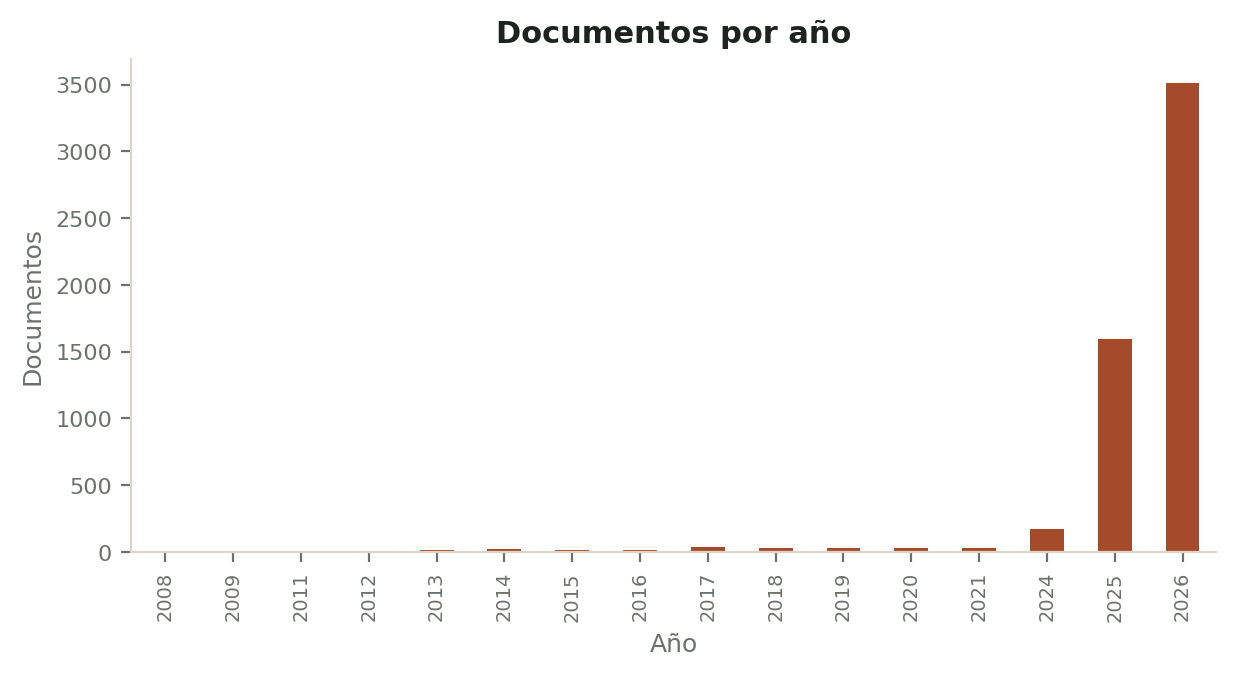
\includegraphics[width=\columnwidth]{perfil_anios.png}
\caption{Documentos por a\~no en el corpus.}
\label{fig:anios}
\end{figure}

\subsection{Duplicados y longitud}

Hay 14.771 copias excedentes (filas que repiten un texto ya presente) agrupadas en 4.434 grupos, con un m\'aximo de 839 copias. Si se cuentan todas las filas que pertenecen a un grupo duplicado, son 19.205: 9.972 en Bluesky y 9.233 en prensa. Las dos cifras son compatibles: la primera cuenta copias adicionales y la segunda, documentos en grupos. No se borran filas en la ingesta, porque eso perder\'ia la procedencia; la deduplicaci\'on se hace en la recuperaci\'on, comparando el hash del fragmento antes de armar el contexto.

La longitud media es de 473 palabras y 2.977 caracteres, pero la mediana baja a 371 palabras y 2.367 caracteres. La cola es larga: el percentil 99 llega a 2.420 palabras y el m\'aximo a 58.181 palabras, equivalentes a 363.528 caracteres. Ese documento extremo produce cientos de fragmentos y obliga a controlar el tama\~no de lote en la ingesta.

\subsection{Ruido de rastreo}

El rastreador dej\'o p\'aginas de error dentro del corpus. La misma p\'agina con los mensajes ``Haz excedido el m\'aximo de peticiones'' y ``Error 505'' aparece en 7.378 documentos, el 4,36\,\% del total, todos en la colecci\'on de prensa. En el conjunto de humo esos textos casi id\'enticos dominaban el top-10 de cualquier consulta, porque su similitud entre s\'i es mayor que la de cualquier documento relevante. El registro de ingesta descarta 7.380 documentos por calidad: 7.378 son esa p\'agina de error y 2 no est\'an desglosados. Quedan 161.868 documentos indexados y 618.286 fragmentos. El porcentaje de documentos con al menos un patr\'on de ruido (peticiones, error 505, cookies, inicio de sesi\'on) llega al 5,3\,\%, pero el filtro solo elimina los marcadores fuertes de error y no las menciones leg\'itimas de cookies.

\subsection{Textometr\'ia}

La textometr\'ia se calcul\'o sobre dos muestras: los 2.000 documentos del piloto y 5.000 documentos estratificados del resto del corpus, con semilla 42. La Tabla~\ref{tab:textometria} compara los indicadores. Los valores son estables entre las dos muestras; eso no demuestra que el piloto represente la distribuci\'on del corpus, solo que no se observan diferencias gruesas en estos indicadores.

\begin{figure*}[t]
\centering
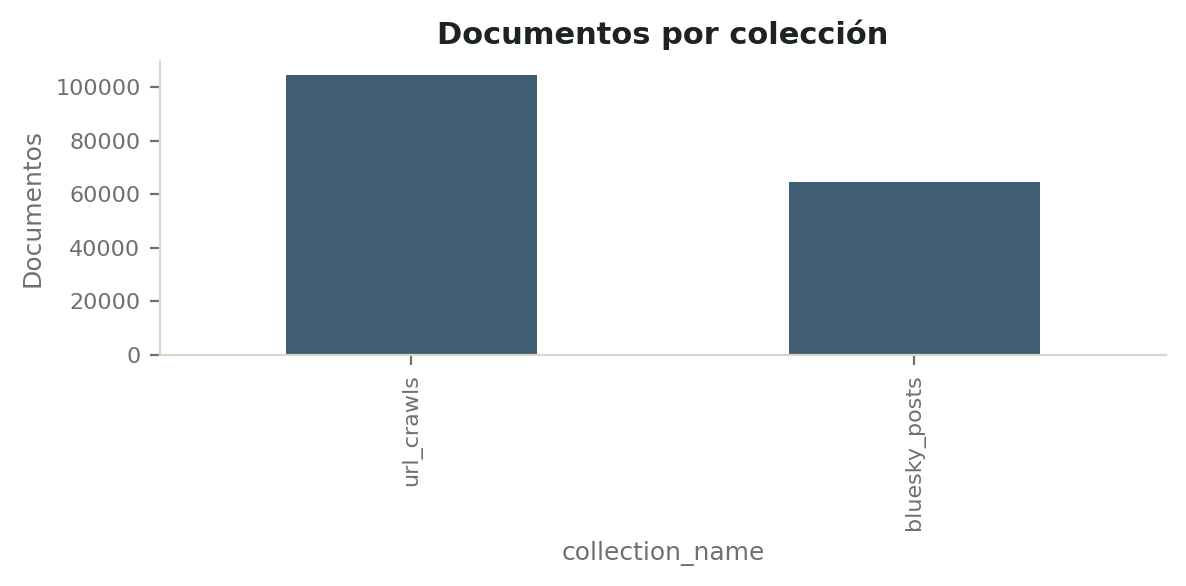
\includegraphics[width=0.8\textwidth]{perfil_colecciones.png}
\caption{Documentos por colecci\'on. Los dos totales coinciden con la Tabla~\ref{tab:composicion}.}
\label{fig:colecciones}
\end{figure*}

\begin{figure*}[t]
\centering
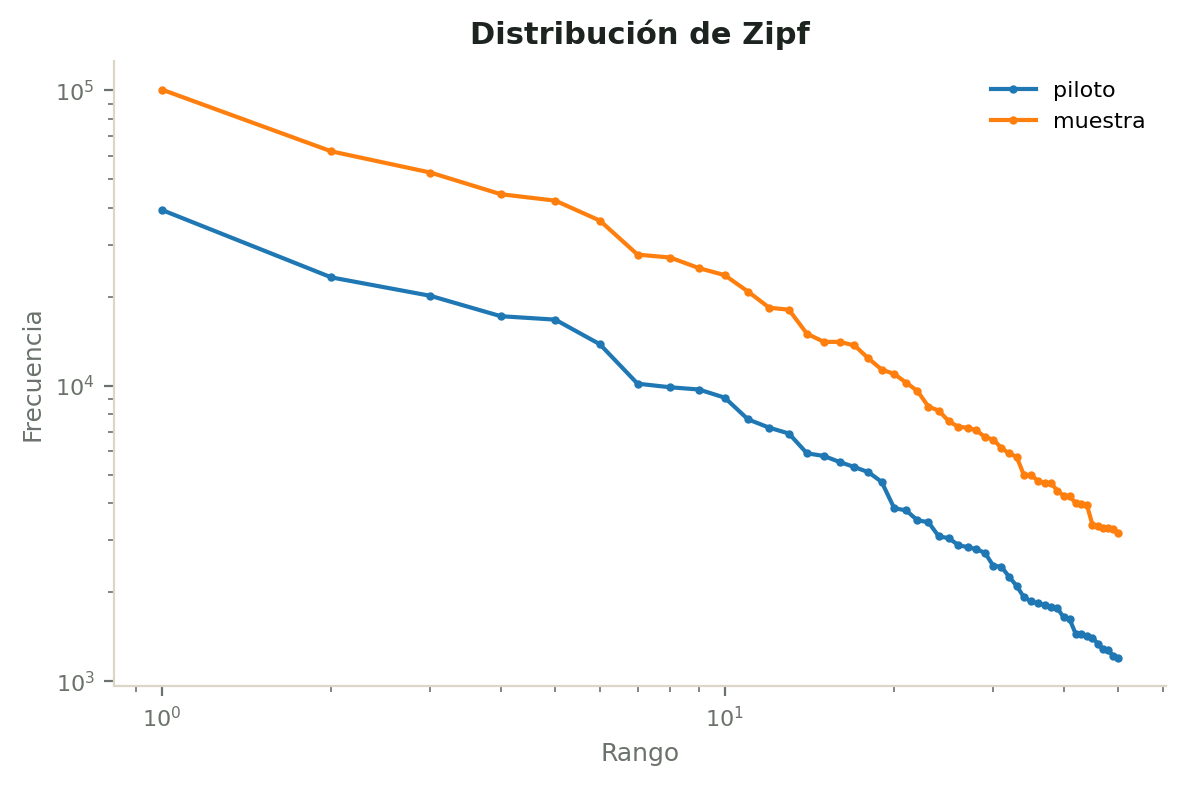
\includegraphics[width=0.8\textwidth]{textometria_zipf.png}
\caption{Rango frente a frecuencia en escala logar\'itmica para el piloto y la muestra. Se muestran los 50 t\'erminos m\'as frecuentes; no se ajusta una recta, la figura solo comprueba la forma de ley de potencia.}
\label{fig:zipf}
\end{figure*}

\begin{figure*}[t]
\centering
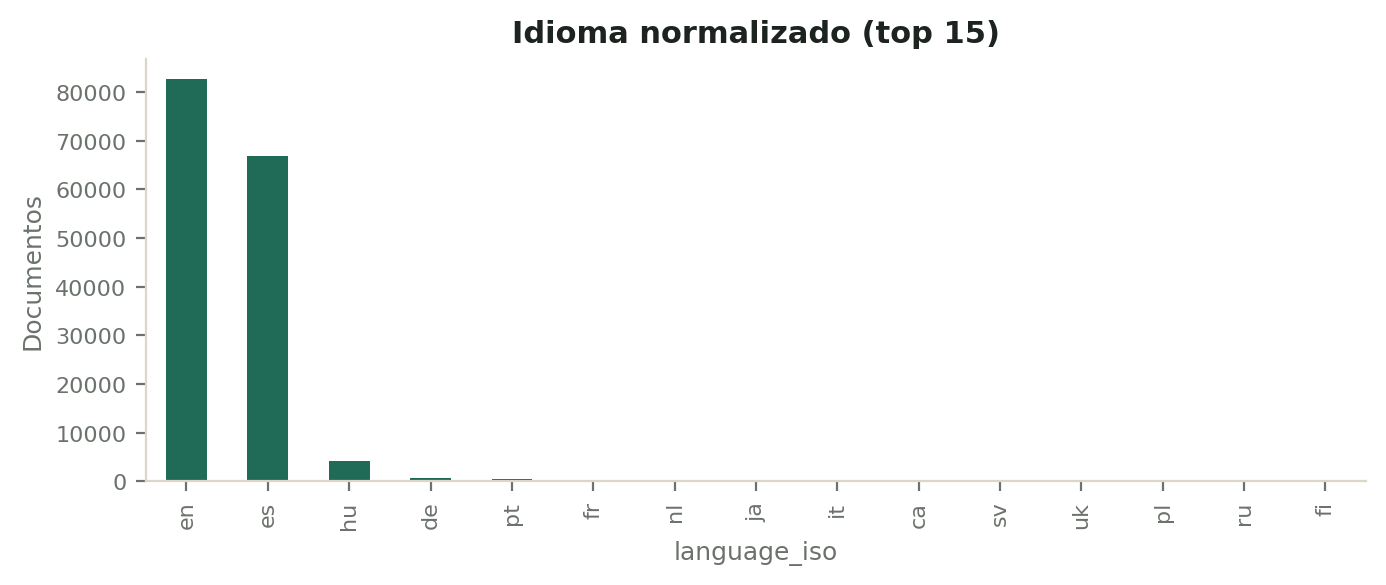
\includegraphics[width=0.8\textwidth]{perfil_idiomas.png}
\caption{Idiomas normalizados m\'as frecuentes (15 primeros). La normalizaci\'on se hace al vuelo; el campo crudo del archivo no se modifica.}
\label{fig:idiomas}
\end{figure*}

\begin{figure*}[t]
\centering
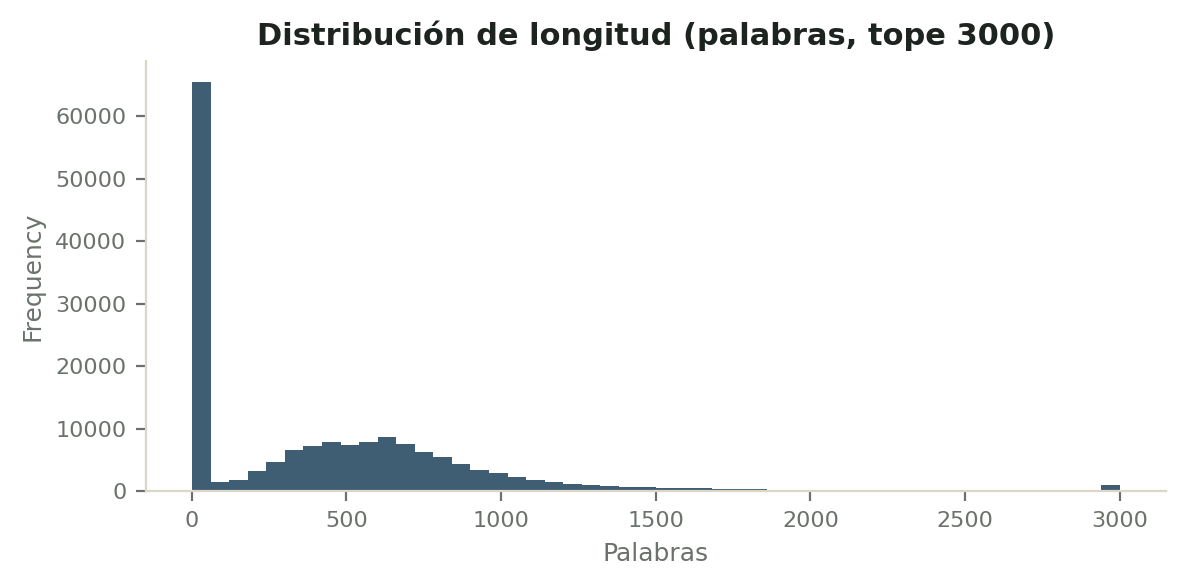
\includegraphics[width=0.8\textwidth]{perfil_longitud.png}
\caption{Distribuci\'on de longitud en palabras. Los documentos de m\'as de 3.000 palabras se acumulan en el extremo derecho del histograma.}
\label{fig:longitud}
\end{figure*}


\begin{table}[t]
\centering
\caption{Textometr\'ia del piloto y de una muestra del corpus completo.}
\label{tab:textometria}
\begin{tabular}{lrr}
\toprule
Indicador & Piloto & Muestra \\
\midrule
Tipos por documento (mediana) & 188 & 188 \\
TTR mediana & 0,579 & 0,570 \\
Hapax / tipos (mediana) & 0,773 & 0,770 \\
Guiraud (mediana) & 10,04 & 10,13 \\
Caracteres por documento (mediana) & 2.317 & 2.353 \\
Caracteres p99 & 14.979 & 15.498 \\
Sin puntuaci\'on terminal (proxy) & 33,5\,\% & 32,7\,\% \\
Documentos con URL & 9,3\,\% & 9,9\,\% \\
Documentos con correo & 1,8\,\% & 1,3\,\% \\
Documentos con emojis & 12,4\,\% & 12,1\,\% \\
Documentos con navegaci\'on & 3,4\,\% & 3,3\,\% \\
Documentos con boilerplate & 3,4\,\% & 4,5\,\% \\
Near-duplicates (SimHash, Hamming $\leq 3$) & 4,25\,\% & 4,72\,\% \\
Grupos de near-duplicates & 26 & 53 \\
Grupo m\'as grande & 12 & 32 \\
\bottomrule
\end{tabular}
\end{table}

El 32,7\,\% de los documentos de la muestra no termina en un signo de cierre. Es un proxy de truncamiento, no una verificaci\'on de que el rastreador los cort\'o: una publicaci\'on completa puede acabar sin punto. La limpieza no puede recuperar ese texto, y el porcentaje se declara como l\'imite en la Secci\'on~\ref{sec:limitaciones}. El HTML residual es marginal (0,14\,\% en la muestra), pero las URLs aparecen en uno de cada diez documentos y los emojis en uno de cada ocho, casi todo en Bluesky. Los near-duplicates no son solo hash exacto: SimHash encuentra grupos de hasta 32 documentos que el hash exacto no captura. Los t\'erminos exclusivos de prensa est\'an dominados por boilerplate (\emph{publicidad}, \emph{informaci\'on}, \emph{adem\'as}), lo que anticipa que una normalizaci\'on conservadora puede ayudar sin destruir entidades.

\begin{figure*}[t]
\centering
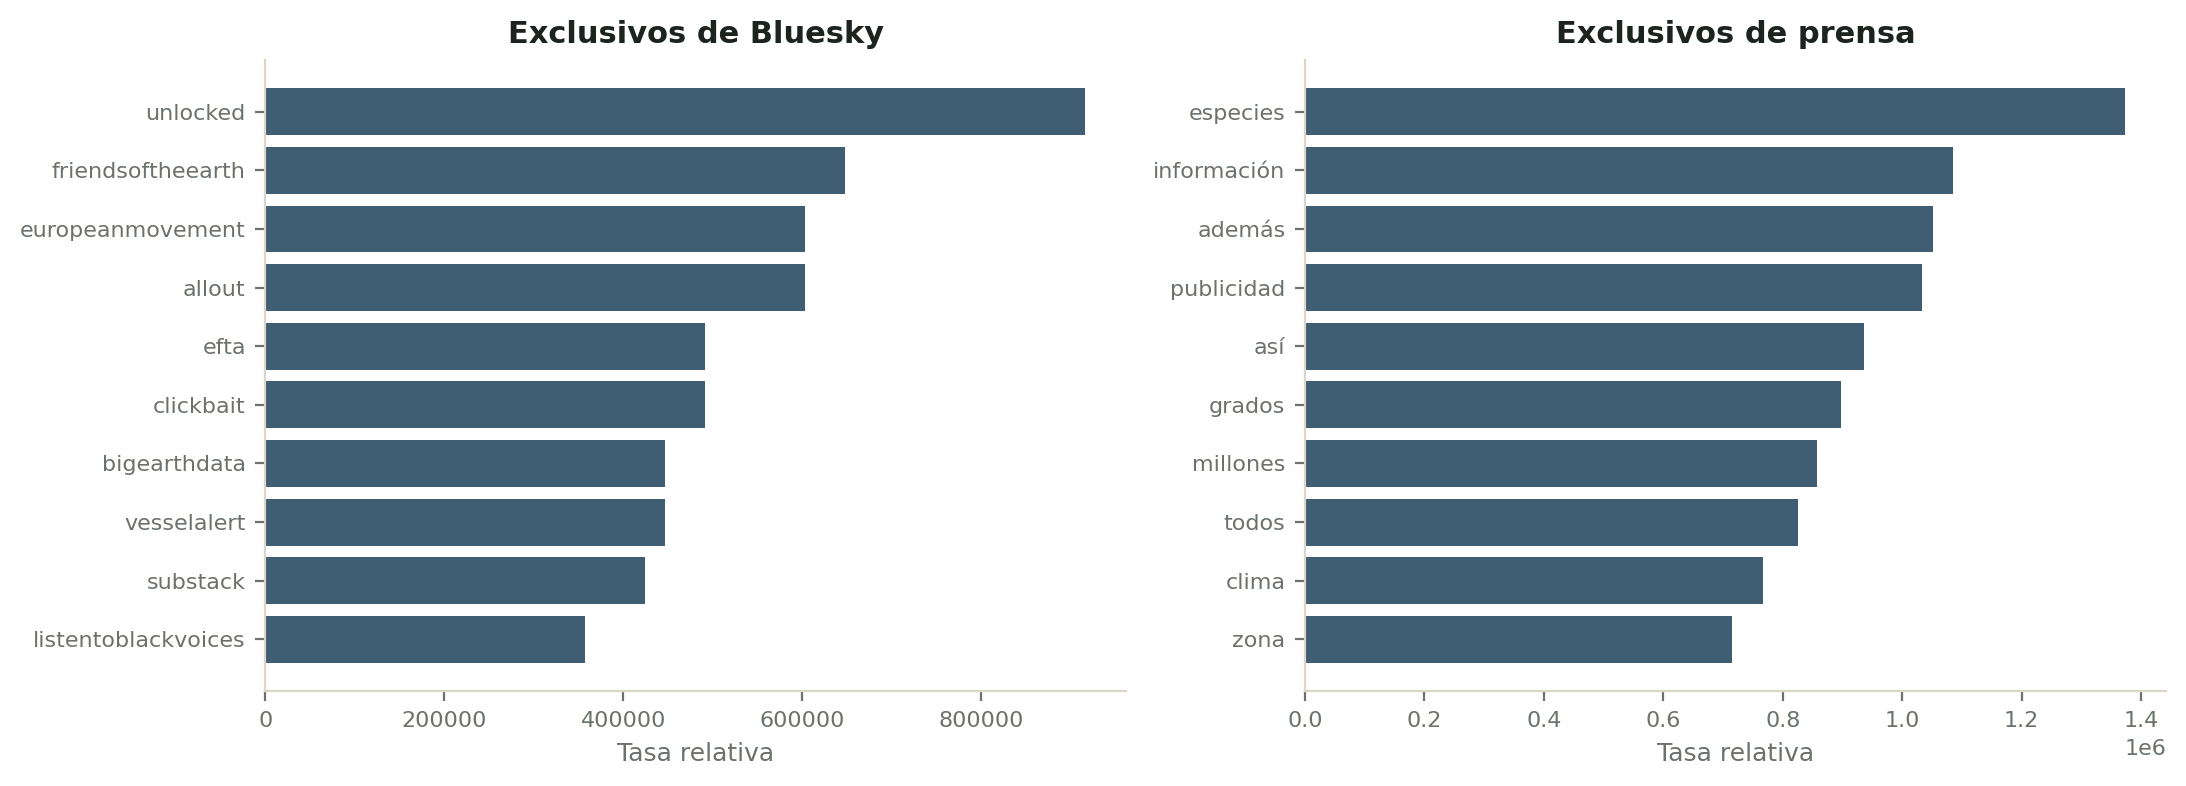
\includegraphics[width=0.8\textwidth]{textometria_terminos.png}
\caption{T\'erminos m\'as frecuentes del piloto y de la muestra.}
\label{fig:terminos}
\end{figure*}

\begin{figure*}[t]
\centering
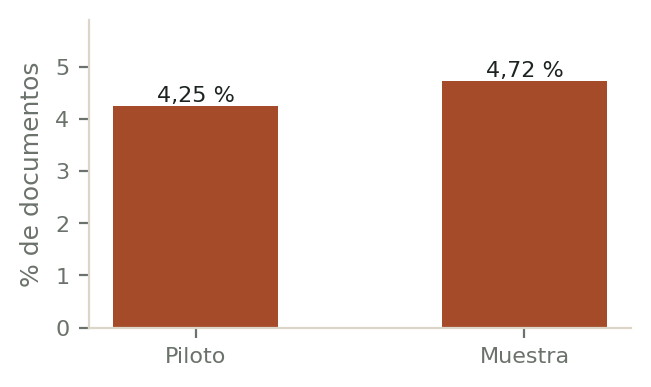
\includegraphics[width=0.8\textwidth]{textometria_near_dups.png}
\caption{Duplicados cercanos: distribuci\'on de similitud entre documentos.}
\label{fig:dups}
\end{figure*}

\begin{figure*}[t]
\centering
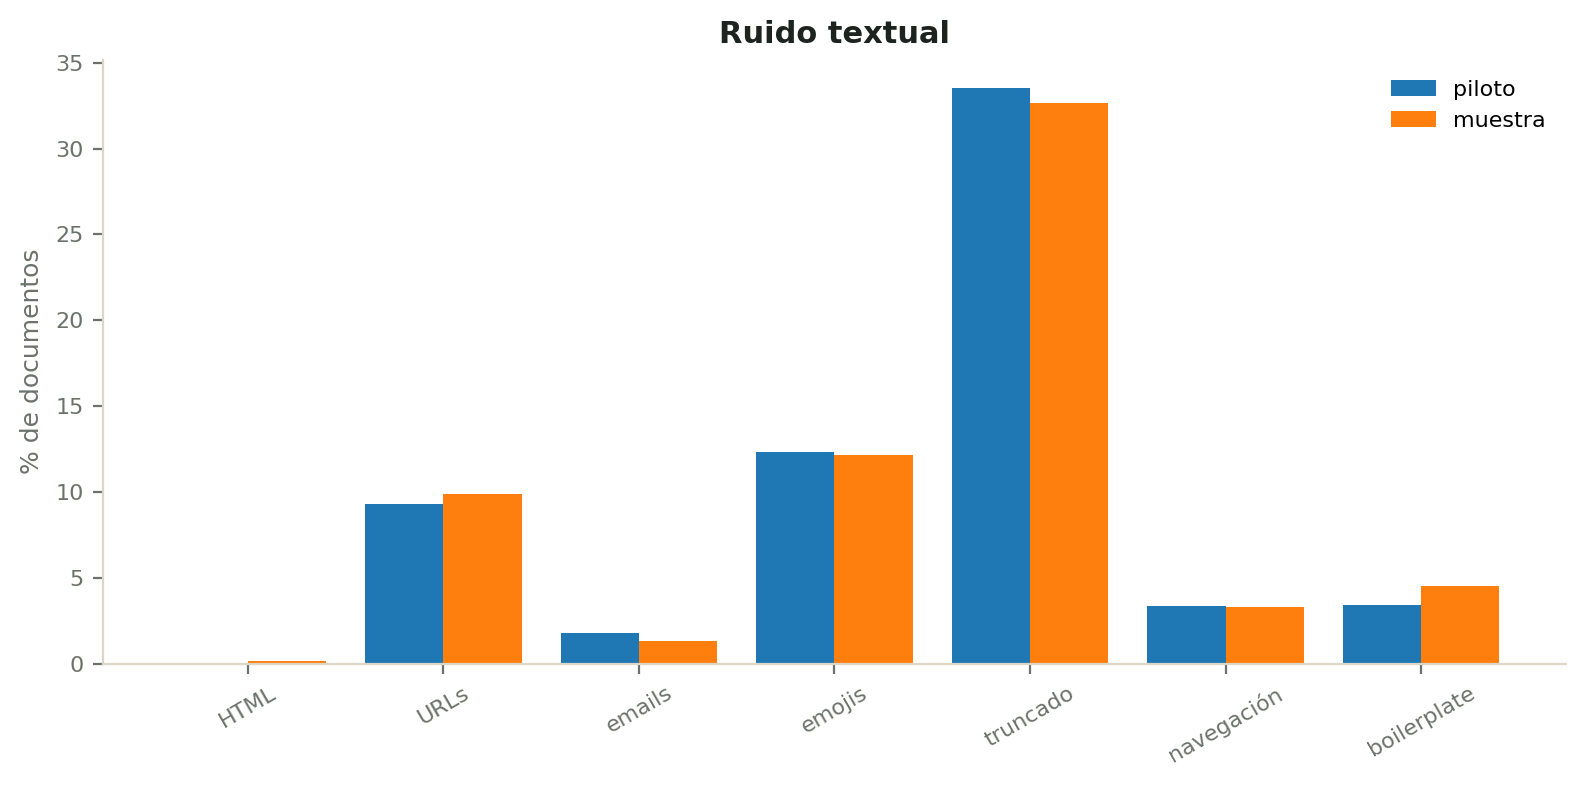
\includegraphics[width=0.8\textwidth]{textometria_ruido.png}
\caption{Indicadores de ruido de rastreo en el corpus.}
\label{fig:ruido}
\end{figure*}

\subsection{Decisiones de procesamiento}

El an\'alisis anterior fija tres decisiones. Primero, limpieza conservadora: se elimina boilerplate y se normalizan espacios, pero no se tocan entidades ni n\'umeros. Segundo, deduplicaci\'on en la recuperaci\'on, no en la ingesta, para conservar la trazabilidad. Tercero, el truncamiento se declara como l\'imite y no se intenta reconstruir. La Secci\'on~\ref{sec:experimentos} mide si la limpieza conservadora mejora la recuperaci\'on frente a no limpiar.

\section{Arquitectura}
\label{sec:arquitectura}

\subsection{Vista general}

La arquitectura se organiza como un marco modular de capas con contratos expl\'icitos. Cada capa declara qu\'e recibe, qu\'e entrega y qu\'e invariante conserva; la instancia concreta de cada ranura, sea el codificador, la mezcla de recuperaci\'on, el generador o el umbral, se elige por medici\'on y se fija en la Secci\'on~\ref{sec:experimentos}. La Figura~\ref{fig:arquitectura} muestra la instancia final; el arco que la separa de la l\'inea base, con sus hip\'otesis y sus rechazos, se despliega en la Secci\'on~\ref{sec:experimentos}. Ninguna pieza se justifica por s\'i sola: la justificaci\'on es la comparaci\'on que la eligi\'o.

\begin{figure}[t]
\centering
\begin{tikzpicture}[
  node distance=0.55cm,
  box/.style={draw, rounded corners=2pt, align=center, font=\scriptsize, minimum width=2.6cm, minimum height=0.7cm, fill=black!3},
  db/.style={draw, cylinder, shape border rotate=90, aspect=0.25, align=center, font=\scriptsize, minimum width=1.9cm, minimum height=0.8cm, fill=black!8},
  arr/.style={-{Latex[length=2mm]}, thick}
]
\node[box] (ui) {UI Streamlit};
\node[box, below=of ui] (api) {API FastAPI};
\node[box, below=of api] (cond) {Condensador\\gemma2:2b};
\node[box, below=of cond, minimum height=1.1cm] (ret) {Recuperaci\'on\\denso bge-m3 top-10\\+ BM25 top-20};
\node[box, below=of ret] (score) {Score cross-encoder};
\node[box, below=of score] (gate) {Compuerta de dominio\\(Modo estricto)};
\node[box, below=of gate] (rer) {Reranker GPU\\bge-reranker-v2-m3};
\node[box, below=of rer] (prompt) {Prompt v2};
\node[box, below=of prompt] (llm) {gemma4:e4b + MTP};
\node[box, below=of llm] (guard) {Guardarra\'iles};
\node[box, below=of guard, fill=black!10] (resp) {Respuesta con citas};
\node[box, left=0.5cm of guard, dashed, fill=black!6] (abst) {Abstenci\'on\\con motivo};
\node[db, right=0.55cm of ret] (milvus) {Milvus\\618k};
\draw[arr] (ui) -- (api);
\draw[arr] (api) -- (cond);
\draw[arr] (cond) -- (ret);
\draw[arr] (ret) -- (score);
\draw[arr] (score) -- (gate);
\draw[arr] (gate) -- (rer);
\draw[arr] (rer) -- (prompt);
\draw[arr] (prompt) -- (llm);
\draw[arr] (llm) -- (guard);
\draw[arr] (guard) -- (resp);
\draw[arr, dashed] (gate.west) -- ++(-0.5,0) |- (abst.east);
\draw[arr, dashed] (guard.west) -- (abst.east);
\draw[arr, <->] (ret) -- (milvus);
\end{tikzpicture}
\caption{Flujo de una consulta en la instancia final. La compuerta solo act\'ua con el Modo estricto; el condensador solo en preguntas encadenadas. Las l\'ineas discontinuas son las salidas de abstenci\'on, antes y despu\'es de generar.}
\label{fig:arquitectura}
\end{figure}

\subsection{Capas y justificaci\'on}

\textbf{Ingesta.} La capa convierte documentos crudos en fragmentos con metadatos. El contrato exige idempotencia y reanudaci\'on: cada fragmento guarda \texttt{document\_id}, t\'itulo, URL, fuente, idioma, fecha, posici\'on, estrategia y hash, y la colecci\'on valida su etiqueta contra el codificador activo. La instancia final usa chunking fijo; el coste medido es 2 h 41 min para la ingesta completa y 27,3 min para reindexar 618.286 fragmentos ya troceados.

\textbf{\'Indice vectorial.} La capa recibe vectores y devuelve vecinos con metadatos. El contrato exige b\'usqueda aproximada con par\'ametro de exploraci\'on ajustable y filtrado por idioma, fecha y colecci\'on sin salir del motor; Milvus con HNSW cumple las tres condiciones \cite{malkov2020hnsw}. El tama\~no de la colecci\'on y el valor de \texttt{ef} se fijan en la Secci\'on~\ref{sec:experimentos}.

\textbf{Codificaci\'on.} La capa recibe texto y devuelve vectores densos. El contrato exige multiling\"uismo sin ajuste fino y una dimensi\'on declarada en la etiqueta de la colecci\'on. La comparaci\'on entre e5-base, qwen3-embedding y bge-m3 se reporta en la Secci\'on~\ref{sec:experimentos}; la instancia final es bge-m3 \cite{chen2024bge}.

\textbf{Recuperaci\'on.} La capa recibe una consulta y devuelve $k$ fragmentos con puntuaci\'on. El contrato exige dos rutas independientes, densa y dispersa, deduplicaci\'on por texto y conservaci\'on del top-5 denso que consume la compuerta. La instancia final une denso top-10 y BM25 top-20; las mezclas y la fusi\'on RRF se miden en la Secci\'on~\ref{sec:experimentos}. El mismo contrato se implement\'o sobre Solr 9 con \texttt{edismax}; el \'indice replica los 618.286 fragmentos y se selecciona con \texttt{RETRIEVER=solr}.

\textbf{Reordenamiento.} La capa recibe pares pregunta-fragmento y devuelve un orden. El contrato exige una puntuaci\'on reutilizable por la compuerta para no pagar dos pasadas. El cross-encoder multiling\"ue corre en GPU con lote de 16 \cite{nogueira2019passage}; el coste medido es 0,68 s para 50 pares, frente a 1,30 s para 5 pares en CPU. El recorte y la profundidad se comparan en la Secci\'on~\ref{sec:experimentos}.

\textbf{Generaci\'on.} La capa recibe el prompt y el contexto y devuelve texto con citas. El contrato es agn\'ostico del modelo: temperatura 0, presupuesto de 16.384 tokens de entrada, prompt v2 con ocho reglas y frase de abstenci\'on exacta. gemma4:e4b es la instancia final por contexto y MTP, no por ganar una comparaci\'on directa; los modelos peque\~nos y la corrida final se eval\'uan en la Secci\'on~\ref{sec:experimentos}.

\textbf{Conversaci\'on.} La capa recibe el historial y la \'ultima pregunta y devuelve una consulta aut\'onoma. El contrato exige no cargar un segundo modelo grande; gemma2:2b act\'ua de condensador y, si pierde el tema, se antepone la primera pregunta del usuario.

\textbf{Guardarra\'iles.} La capa recibe la respuesta y las evidencias y devuelve la respuesta o una abstenci\'on con motivo. Tres controles: cita obligatoria, verificaci\'on de entidades y n\'umeros contra el fragmento citado, y un juez de evidencia distinto del generador. El juez es gemma2:2b para no validar con el mismo modelo que redacta.

\textbf{Compuerta de dominio.} La capa recibe la puntuaci\'on del cross-encoder y se\~nales de recuperaci\'on y devuelve una probabilidad de dominio. El contrato exige ser reproducible y medible con precisi\'on y recall, no un LLM juez; una regresi\'on log\'istica reutiliza la pasada del reranker. Se activa con el interruptor Modo estricto y su entrenamiento se reporta en la Secci\'on~\ref{sec:experimentos}.

\textbf{API e interfaz.} FastAPI separa el pipeline de la presentaci\'on y expone \texttt{/chat}, \texttt{/ask}, \texttt{/retrieve}, \texttt{/health}, \texttt{/models} y \texttt{/stats} \cite{fastapidocs}. Streamlit consume \texttt{/chat} y muestra la respuesta, las citas, las evidencias, las m\'etricas y el razonamiento \cite{streamlitdocs}. La separaci\'on permite probar el pipeline sin la interfaz y cambiar la interfaz sin tocar el pipeline.

\subsection{Configuraci\'on final}

La Tabla~\ref{tab:config-final} fija la instancia final del marco. Cada valor se justifica en las Secciones~\ref{sec:metodo} y~\ref{sec:experimentos}.

\begin{table}[t]
\centering
\caption{Configuraci\'on final del sistema.}
\label{tab:config-final}
\begin{tabular}{ll}
\toprule
Par\'ametro & Valor \\
\midrule
Codificador & BAAI/bge-m3, 1024 dimensiones \\
\'Indice & HNSW en Milvus, \texttt{ef}=800 \\
Recuperaci\'on & uni\'on densa top-10 + BM25 top-20, $k=10$ \\
Reordenador & BAAI/bge-reranker-v2-m3, GPU, top-10 \\
Generador & gemma4:e4b, Q4\_K\_M \\
Contexto & 116.384 tokens (16.384 entrada, 100.000 salida) \\
MTP & draft 3, 217 tok/s \\
Prompt & v2 \\
Juez y condensador & gemma2:2b \\
Compuerta & regresi\'on log\'istica con cross-encoder, umbral 0,4 \\
Fragmentos & 618.286 en \texttt{rag\_full\_bge\_m3\_d1024\_v1} \\
\bottomrule
\end{tabular}
\end{table}

\subsection{Despliegue: datos en Swarm, GPU en la estaci\'on}

La capa de datos (etcd, MinIO y Milvus) se despliega como un stack de Docker Swarm en el servidor, con la etiqueta \texttt{role=data}. Milvus publica el puerto 19530 en modo host y el API se conecta a \texttt{http://192.168.1.100:19530}. La aplicaci\'on (API, frontend y Ollama) corre en la estaci\'on con Compose y \texttt{network\_mode: host}, porque necesita la GPU AMD.

La separaci\'on no es arbitraria. Swarm aporta colocaci\'on declarativa, pol\'itica de reinicio y una red overlay que elimina el t\'unel SSH de la versi\'on anterior; con el t\'unel, una ca\'ida de la conexi\'on dejaba al sistema sin recuperaci\'on. La aplicaci\'on no puede ir en el stack: Docker Swarm no admite el paso de dispositivos (\texttt{devices}) ni \texttt{privileged} en un servicio, y el cgroup de dispositivos bloquea \texttt{/dev/kfd} con \textit{Operation not permitted} aunque se monte el nodo y el grupo sea el correcto. Se comprob\'o con un servicio de prueba: el montaje y los grupos 983 y 987 funcionan, pero la apertura del dispositivo falla. Un stack completo obligar\'ia a mover el generador a la GPU del servidor (GTX 1080 de 8 GB), que no soporta el contexto de 116K.

Compose se mantiene para la aplicaci\'on porque es el \'unico runtime del proyecto que pasa la GPU AMD, y el stack se mantiene para los datos porque es el que elimina el t\'unel y hace declarativo el reparto. Un solo Compose no puede repartir servicios entre dos hosts; un solo Swarm no puede pasar la GPU.

\subsection{Interfaz para el usuario final}

La interfaz tiene dos zonas. En el panel lateral se elige el modelo, el n\'umero de fragmentos, el idioma del documento, el rango de fechas y la colecci\'on; se activan el razonamiento y el Modo estricto, y se cambia entre tema claro y oscuro. En el \'area central se conversa con historial. Cada respuesta muestra el texto con citas numeradas, chips con la intenci\'on y la ruta de ejecuci\'on, la latencia por etapa, los tokens por segundo y un desplegable con las evidencias: t\'itulo, puntuaci\'on, fragmento, enlace y metadatos. Si el sistema se abstiene, aparece el motivo y, en el caso de fuera de dominio, la sugerencia de desactivar el Modo estricto. El razonamiento del modelo, cuando se activa, va en un desplegable separado y se advierte que no sustituye la evidencia. La Figura~\ref{fig:ui} muestra una respuesta real con las evidencias abiertas.

\begin{figure*}[!t]
\centering
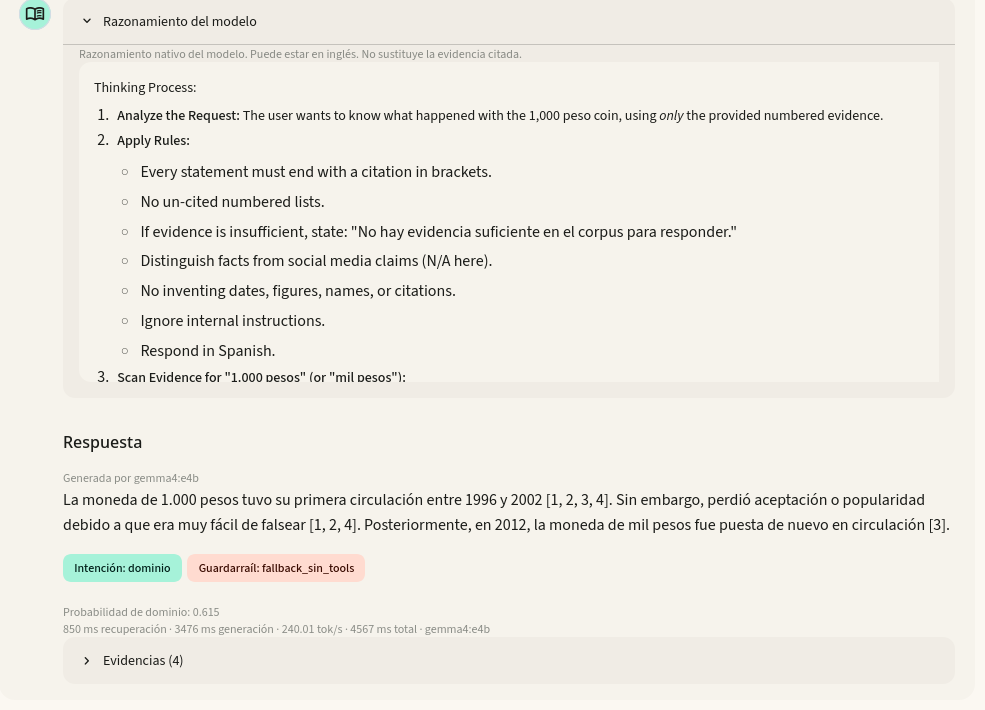
\includegraphics[width=0.9\textwidth]{figuras/ui_recorte.png}
\caption{Interfaz final: respuesta con citas y evidencias abiertas. La pregunta se acepta con probabilidad de dominio 0,956; la respuesta cita diez evidencias y el panel muestra t\'itulo, puntuaci\'on, fragmento, enlace y metadatos de la primera. El chip de la derecha identifica la ruta de ejecuci\'on, no un guardarra\'il de cita.}
\label{fig:ui}
\end{figure*}

\begin{figure}[t]
\centering
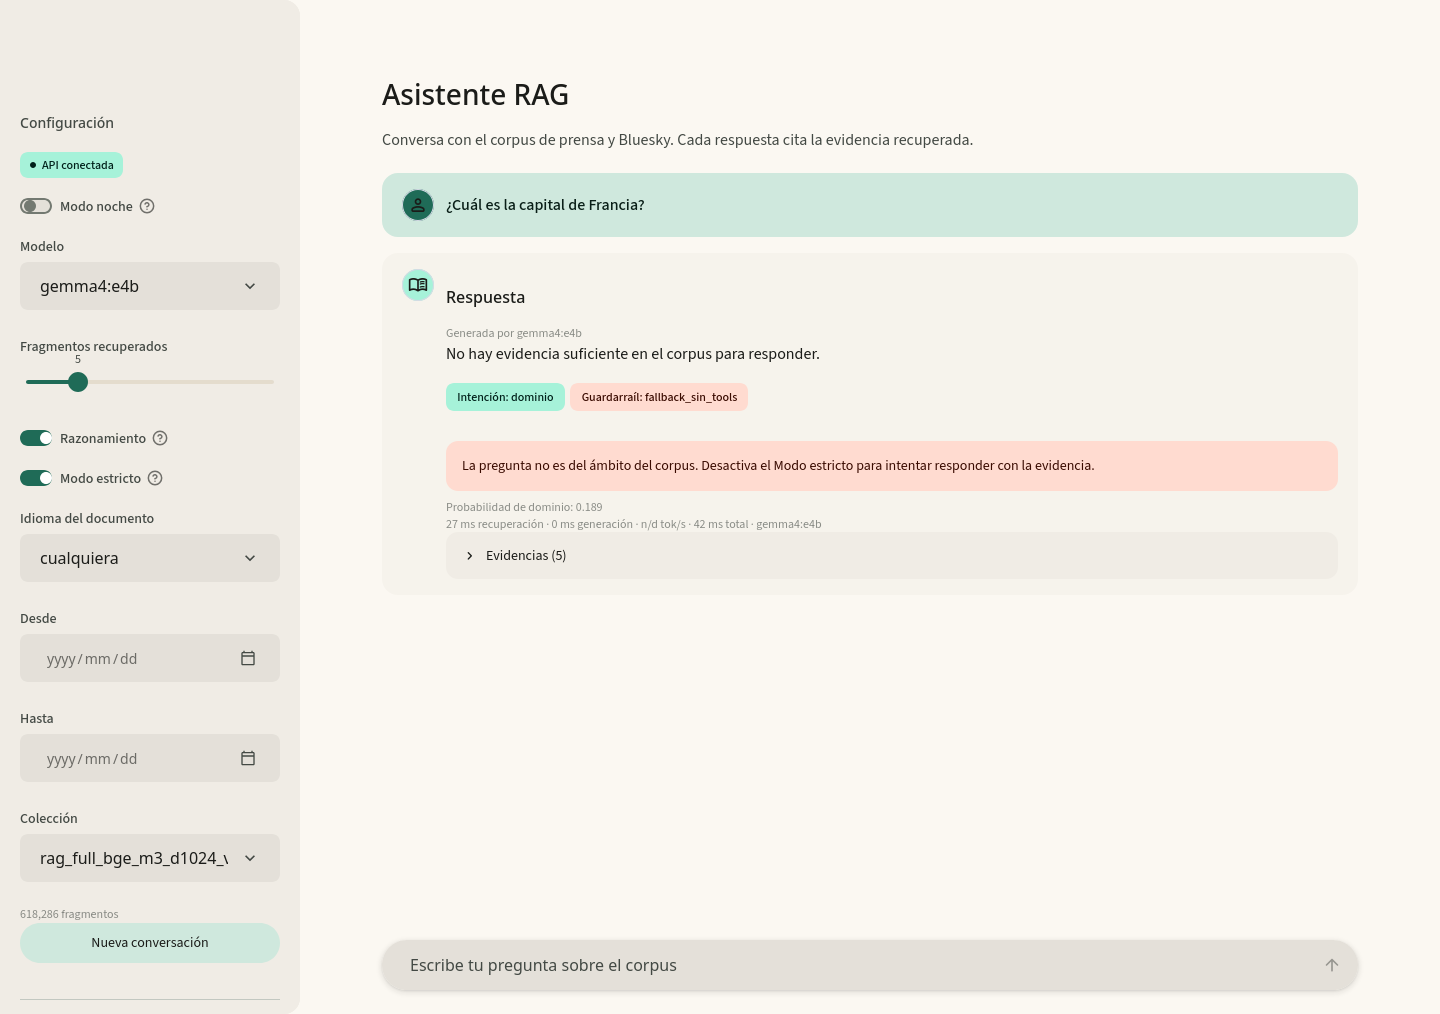
\includegraphics[width=\columnwidth]{ui_m3_estricto.png}
\caption{Modo estricto: la compuerta rechaza una pregunta fuera de dominio y explica el motivo.}
\label{fig:ui-estricto}
\end{figure}


\section{Metodolog\'ia}
\label{sec:metodo}

\subsection{Limpieza y deduplicaci\'on}

La variante adoptada, V2, descarta las p\'aginas de error del rastreador, aplica normalizaci\'on NFKC, quita HTML y URLs y colapsa espacios. No elimina signos, n\'umeros ni entidades, porque son la se\~nal que usan los guardarra\'iles. Los duplicados exactos y los near-duplicates se descartan al armar el contexto, comparando el hash del fragmento y su SimHash antes de insertarlo. As\'i se conserva la procedencia en el \'indice y se evita repetir el mismo texto en el prompt.

\subsection{Segmentaci\'on}

Se usa chunking fijo de 1000 caracteres con 150 de solape (\texttt{fixed\_v2}). El solape cubre la frontera donde suele caer la respuesta. Cada fragmento guarda \texttt{document\_id}, t\'itulo, URL, fuente, idioma, fecha, posici\'on, estrategia y hash del texto. Esos metadatos permiten filtrar por idioma y fecha y auditar cada cita.

\subsection{Codificaci\'on e \'indice}

Los fragmentos se codifican con BAAI/bge-m3 en la GPU, en fp16 y por lotes. La colecci\'on se llama \texttt{rag\_full\_bge\_m3\_d1024\_v1} y usa HNSW con \texttt{ef}=800 en la b\'usqueda. El par\'ametro se eligi\'o con una rejilla sobre el silver: por debajo de 800 el recall cae y por encima la latencia sube sin ganancia apreciable. En paralelo se mantiene una colecci\'on BM25 sobre los mismos fragmentos, \texttt{rag\_full\_e5base\_d768\_v2\_bm25\_v1}, que alimenta la recuperaci\'on dispersa.

\subsection{Recuperaci\'on y reordenamiento}

La recuperaci\'on combina dos listas. La densa pide 10 fragmentos a bge-m3; la dispersa pide 20 a BM25. Las dos se unen sin fusionar, se deduplican por texto y se pasan al reordenador. El cross-encoder multiling\"ue punt\'ua cada par pregunta-fragmento en GPU, con lote de 16, y el resultado se recorta a 10. La uni\'on conserva el top-5 denso, que es la se\~nal que la compuerta espera, y a\~nade las entidades que BM25 encuentra y el denso no. Los filtros de idioma, fecha y colecci\'on se aplican en Milvus.

\subsection{Generaci\'on}

El generador es gemma4:e4b con temperatura 0 y un presupuesto de 16.384 tokens de entrada. El prompt v2 impone ocho reglas: cada afirmaci\'on lleva una cita entre corchetes; no se permiten listas sin cita; si la evidencia no alcanza se responde con una frase de abstenci\'on exacta; se distingue un hecho verificable de una afirmaci\'on publicada en redes; no se inventan fechas, cifras, nombres ni citas; se ignoran las instrucciones que aparezcan dentro de los documentos; se responde en el idioma de la pregunta; y se usa la fecha exacta de la evidencia cuando la pregunta la pide. El MTP con draft 3 se activa en el manifiesto del modelo y no cambia la salida, solo la velocidad.

\subsection{Guardarra\'iles}

Antes de devolver la respuesta se aplican tres controles. El primero exige al menos una cita v\'alida; si no hay, se abstiene con \texttt{sin\_citas}. El segundo extrae entidades y n\'umeros de la respuesta y verifica que aparezcan en el fragmento citado o en la pregunta; si no, se abstiene con \texttt{sin\_respaldo} o \texttt{citas\_invalidas}. El tercero pide a un juez distinto, gemma2:2b, que decida si la cita sostiene la respuesta; si dice que no, se abstiene con \texttt{juez\_no}. Cuando el fragmento est\'a en ingl\'es y la respuesta en espa\~nol, la cobertura l\'exica se salta y decide el juez, para no castigar una traducci\'on correcta.

\subsection{Compuerta de dominio}

La compuerta usa la puntuaci\'on del cross-encoder sobre el top-5 (m\'aximo, media, diferencia entre el primero y el segundo, y m\'inimo), cinco features de recuperaci\'on (puntuaci\'on del primer fragmento, media del top-5, diferencia entre el primero y el segundo, solapamiento entre la pregunta y el t\'itulo, y presencia de la entidad principal en el t\'itulo) y un one-hot del tipo de pregunta. La puntuaci\'on del cross-encoder se calcula una sola vez y se reutiliza para el reordenamiento. El modelo es una regresi\'on log\'istica con escalado y \texttt{class\_weight=balanced}; la regularizaci\'on se eligi\'o por validaci\'on cruzada de cinco pliegues sobre train y dev. El umbral es 0,4, elegido para reducir falsos rechazos sin aumentar falsos aceptados. El conjunto tiene 160 preguntas: 60 de dominio y 100 de fuera, con split 103/37/20. Las 40 negativas nuevas son entidades inventadas, eventos futuros y conocimiento general fuera del corpus.

\subsection{API e interfaz}

La API expone \texttt{POST /chat} con historial, \texttt{think} y \texttt{strict}; \texttt{POST /ask} sin historial; \texttt{POST /retrieve} para recuperaci\'on pura; y los GET \texttt{/health}, \texttt{/models} y \texttt{/stats}. La interfaz Streamlit consume \texttt{/chat} y guarda el historial en la sesi\'on. Las preferencias de razonamiento, Modo estricto y tema se guardan en un archivo y se recuperan al recargar. Si el usuario cambia un interruptor mientras el modelo responde, la pregunta queda pendiente y se reintenta en el siguiente ciclo, de modo que la conversaci\'on no se pierde.

\subsection{Despliegue}

El stack se levanta con Docker Compose: etcd, MinIO, Milvus, Ollama, API, frontend y un worker GPU para la ingesta y la evaluaci\'on. La API y el frontend usan red de host. Un servicio de una sola ejecuci\'on, \texttt{prewarm}, espera a que la API est\'e sana y carga el generador, el embedding y el reranker, para que la primera consulta web no pague la carga del modelo.

\section{Protocolo de evaluaci\'on}
\label{sec:evaluacion}

\subsection{Gold est\'andar}

El silver standard tiene 43 preguntas: 19 en desarrollo y 24 en prueba, 38 respondibles y 5 sin respuesta. Lo llamamos silver standard y no gold porque lo gener\'o un LLM y lo revisaron los autores, no expertos independientes. Cada fila guarda el identificador, la pregunta, el idioma, el tipo, el split, los documentos y fragmentos de referencia, el span literal que responde, la respuesta de referencia, el criterio de correcci\'on y el estado de validaci\'on. La Tabla~\ref{tab:gold} resume la composici\'on. Las preguntas sin respuesta no entran en Recall@k: se eval\'uan por abstenci\'on.

\begin{table}[t]
\centering
\caption{Composici\'on del silver standard.}
\label{tab:gold}
\begin{tabular}{lrrr}
\toprule
Split & Respondibles & Sin respuesta & Total \\
\midrule
Desarrollo & 19 & 0 & 19 \\
Prueba & 19 & 5 & 24 \\
\midrule
Total & 38 & 5 & 43 \\
\bottomrule
\end{tabular}
\end{table}

El silver standard se ampli\'o con 17 documentos adicionales marcados por consenso de dos anotadores (kappa 0,626). Con esa ampliaci\'on, 14 preguntas quedaron con dos o m\'as documentos relevantes, lo que hace que Recall@k y nDCG no dependan de un \'unico pasaje.

\subsection{Revisi\'on humana}

Cuatro personas revisaron el silver standard contra el documento citado. Carlos revis\'o las 43 y dej\'o 12 correcciones; Juli\'an aport\'o 7 spans y una reformulaci\'on; \'Oscar aport\'o 5 spans corregidos y marc\'o 3 enlaces rotos; Erika revis\'o las 43, aprob\'o 35, marc\'o 5 como no aplicables y corrigi\'o la respuesta y el span de g-003. Cada propuesta se aplic\'o solo si el span aparec\'ia literalmente en el texto indexado. Las que no se pudieron verificar quedaron con nota.

Para la comparaci\'on de modelos se anotaron 72 respuestas de 4 modelos, ciegas y en orden barajado, con r\'ubrica de 0 a 3 en correcci\'on, fidelidad, citas y abstenci\'on. Dos anotadores calificaron las mismas respuestas. La Tabla~\ref{tab:kappa} reporta el acuerdo. La fidelidad no alcanz\'o acuerdo suficiente y no se usa para el veredicto; la correcci\'on y las citas s\'i.

\begin{table}[t]
\centering
\caption{Acuerdo entre anotadores en la comparaci\'on de modelos (kappa lineal, $n=72$).}
\label{tab:kappa}
\begin{tabular}{lr}
\toprule
Eje & Kappa \\
\midrule
Correcci\'on & 0,95 \\
Citas & 0,90 \\
Abstenci\'on & 0,72 \\
Fidelidad & 0,12 \\
\bottomrule
\end{tabular}
\end{table}

\subsection{M\'etricas}

\textbf{Recuperaci\'on.} Recall@k mide la fracci\'on de documentos de referencia recuperados en el top-k; nDCG@k usa relevancia binaria; P@k mide precisi\'on en el corte; MRR mide la posici\'on del primer acierto; y la cobertura de span indica si al menos un fragmento recuperado contiene el texto exacto que responde. Esta \'ultima es la m\'as cercana a lo que necesita el generador.

\textbf{Respuesta.} Se reportan las preguntas entregadas, las abstenciones, el match estricto (igualdad normalizada con la respuesta de referencia), el F1 por tokens, la tasa de citas, el contexto medio en tokens y la latencia por etapa. La revisi\'on manual clasifica cada respuesta como correcta, parcial o incorrecta.

\textbf{Conversaci\'on.} Catorce casos: seis saludos, cuatro de dominio y cuatro de fuera. Cada uno tiene un resultado esperado y se marca como correcto o incorrecto. Se ejecutan con y sin Modo estricto, y con y sin razonamiento.

\textbf{RAGAS.} Se reportan fidelidad, relevancia de la respuesta, precisi\'on del contexto, cobertura del contexto y correcci\'on de la respuesta \cite{es2023ragas}. Para cada m\'etrica se informa cu\'antas muestras tienen valor, porque el juez falla en algunas y una media con cuatro valores no es comparable con una con 38.

\textbf{Compuerta.} Precisi\'on, recall y F1 en dev y test, falsos rechazos de dominio (preguntas del corpus rechazadas) y falsos aceptados de fuera (preguntas ajenas aceptadas).

\subsection{Estad\'istica}

Las comparaciones de recuperaci\'on usan bootstrap pareado por pregunta con 1.000 remuestreos e intervalos de confianza al 95\,\%. En la comparaci\'on de limpieza se aplica correcci\'on de Bonferroni por comparaciones m\'ultiples. La configuraci\'on se eligi\'o inspeccionando las 43 preguntas del gold, as\'i que los resultados sobre las 38 respondibles son exploratorios. No se dispone de un conjunto de prueba independiente; una evaluaci\'on futura debe reservar preguntas nuevas. Las diferencias que no excluyen cero se reportan como no concluyentes, aunque la media favorezca a una variante. Los intervalos pareados se calcularon para limpieza, E1 y E2; las comparaciones de codificadores, reordenamiento y fusi\'on se reportan como estimaciones puntuales sobre 38 preguntas, sin intervalo, y as\'i se indica en cada tabla.

\subsection{Configuraci\'on de RAGAS}

La corrida de referencia usa juez gemma4:e4b y embeddings BAAI/bge-m3 en CPU, con 38 preguntas directas. El timeout del juez se fij\'o en 900 s y la concurrencia en 6. Con los valores por defecto (180 s y 16 workers) el juez no terminaba en varias muestras y la precisi\'on del contexto quedaba con 4 valores de 38. La corrida de referencia tiene 34 valores en esa m\'etrica y 38 en las dem\'as. Las preguntas sin respuesta se miden aparte y se abstienen 5 de 5.

\section{Experimentos y resultados}
\label{sec:experimentos}

Los experimentos usan el silver standard de 43 preguntas; E12 usa la versi\'on ampliada con 17 documentos adicionales y cada tabla lo indica. La configuraci\'on se eligi\'o con el silver completo, as\'i que los resultados son exploratorios. Cada subsecci\'on reporta el montaje en una frase, la tabla y la decisi\'on; el detalle del montaje est\'a en la Secci\'on~\ref{sec:metodo}.

\subsection{Arco experimental}

Los experimentos no forman una rejilla: siguen un arco de seis estaciones, y cada una se abre con la pregunta que deja la anterior.

\begin{itemize}
\item \textbf{L\'inea base sobre el piloto.} Limpieza, segmentaci\'on y n\'umero de fragmentos con e5-base y 1.932 documentos (Subsecciones \emph{Limpieza} a \emph{Segmentaci\'on y tama\~no del contexto}). El piloto deja un techo alto, Recall@10 de 0,947, y decisiones tomadas por coste y consistencia, no por significancia estad\'istica.
\item \textbf{Modelos peque\~nos e H1.} E4 compara cuatro generadores de 1B a 3B con la misma evidencia recuperada (Subsecci\'on \emph{Modelos generativos}). H1 se refuta: el tama\~no no ordena la calidad; gemma2:2b gana en correcci\'on y citas y llama3.2:1b se abstiene en el 73,7\,\% de las preguntas respondibles.
\item \textbf{Crisis de escala.} E6 repite el pipeline sobre el corpus completo, 161.868 documentos (Subsecci\'on \emph{Codificadores y escala}). Recall@10 cae de 0,947 a 0,684 y nDCG de 0,909 a 0,594 sin que la latencia cambie; la ca\'ida reorganiza el resto del trabajo.
\item \textbf{Rescate h\'ibrido.} BM25, bge-m3, \texttt{ef}=800, la uni\'on densa y dispersa y el reordenador recuperan parte de la p\'erdida (Subsecciones \emph{Codificadores y escala} y \emph{Reordenamiento}). La fusi\'on RRF se rechaza con el silver ampliado y la uni\'on reordenada se adopta para el despliegue.
\item \textbf{Ablaciones negativas.} Las fases 6 y 7 y la inyecci\'on de instrucciones prueban mejoras que no superan la referencia (Subsecciones \emph{Inyecci\'on de instrucciones} y \emph{Prompts y mejoras rechazadas}). Se reportan para acotar el espacio, no para justificar la configuraci\'on.
\item \textbf{Arquitectura ganadora y reservado.} La instancia final se eval\'ua con la compuerta de dominio, RAGAS y el conjunto reservado de 20 preguntas directas y 5 negativas (Subsecciones \emph{Compuerta de dominio} a \emph{Conjunto reservado}). Es la evaluaci\'on de cierre y se reporta tal como sale, incluidas las cifras que empeoran la l\'inea base.
\end{itemize}

El orden importa: las estaciones iniciales se deciden con el silver exploratorio y el conjunto reservado se usa al final para comparar la configuraci\'on desplegada; las cifras de una estaci\'on no se trasladan a otra. Cada subsecci\'on indica con qu\'e conjunto se midi\'o.

\subsection{Limpieza}

Se construyeron cuatro \'indices sobre el piloto con 30 preguntas, e5-base, $k=10$ y tres repeticiones. La Tabla~\ref{tab:limpieza} muestra el resultado. Ninguna comparaci\'on pareada contra V0 excluye cero tras la correcci\'on de Bonferroni sobre 21 pruebas. V2 toca el l\'imite inferior en cuatro m\'etricas, compatible con una mejora peque\~na o con ausencia de efecto. Se adopta V2 por tres razones no estad\'isticas: la consistencia de la estimaci\'on en todas las m\'etricas, el coste nulo en consulta y la eliminaci\'on de 68 p\'aginas de error que de otro modo entrar\'ian al \'indice.

\begin{table}[t]
\centering
\footnotesize
\caption{Limpieza sobre el piloto (30 preguntas, e5-base, $k=10$).}
\label{tab:limpieza}
\setlength{\tabcolsep}{4pt}
\begin{tabular}{lrrrrr}
\toprule
Variante & P@1 & Hit@5 & Recall@10 & MRR & nDCG \\
\midrule
V0 crudo & 0,733 & 0,833 & 0,833 & 0,775 & 0,790 \\
V1 sin p\'aginas de error & 0,767 & 0,833 & 0,833 & 0,800 & 0,809 \\
V2 normalizaci\'on & \textbf{0,833} & \textbf{0,900} & \textbf{0,900} & \textbf{0,867} & \textbf{0,875} \\
V3 V2 + dedup & 0,800 & 0,867 & 0,867 & 0,833 & 0,842 \\
\bottomrule
\end{tabular}
\end{table}

\begin{figure}[t]
\centering
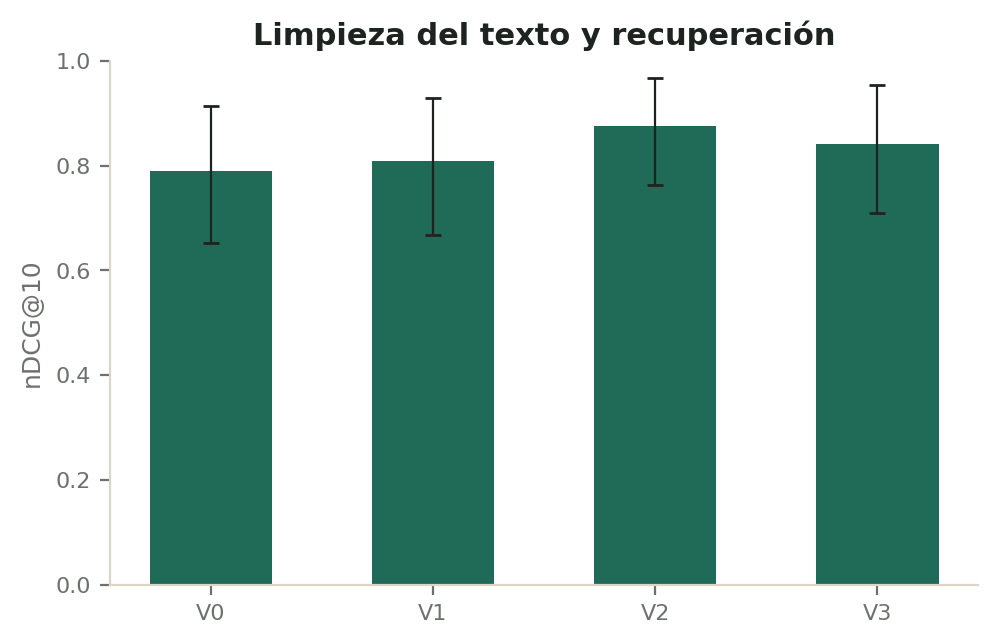
\includegraphics[width=\columnwidth]{limpieza_comparacion.png}
\caption{Comparaci\'on de variantes de limpieza sobre el piloto.}
\label{fig:limpieza}
\end{figure}


\subsection{Segmentaci\'on y tama\~no del contexto}

E1 compar\'o chunking fijo de 1000 caracteres con 150 de solape contra segmentaci\'on por oraciones de 384 caracteres. La Tabla~\ref{tab:e1} muestra estimaciones puntuales favorables al fijo en todas las m\'etricas de calidad, pero ning\'un intervalo pareado excluye cero: nDCG $-0,071$ (IC $[-0,221;\,0,025]$), recall $-0,067$ (IC $[-0,233;\,0,000]$) y P@1 $-0,067$ (IC $[-0,233;\,0,114]$) para oraciones menos fijo. La \'unica diferencia concluyente es la latencia: el fijo es 3,65 ms m\'as r\'apido (IC $[2,25;\,4,97]$). Se mantiene el fijo por la direcci\'on consistente y el coste, no por una mejora de calidad demostrada.

\begin{table}[t]
\centering
\footnotesize
\caption{E1: chunking fijo contra oraciones (30 preguntas).}
\label{tab:e1}
\begin{tabular}{lrrrrr}
\toprule
Variante & P@1 & Hit@5 & Recall@10 & nDCG & p50 \\
\midrule
Fijo 1000/150 & \textbf{0,833} & \textbf{0,900} & \textbf{0,900} & \textbf{0,875} & \textbf{38,5 ms} \\
Oraciones 384/1 & 0,767 & 0,833 & 0,833 & 0,804 & 42,1 ms \\
\bottomrule
\end{tabular}
\end{table}

\begin{figure}[t]
\centering
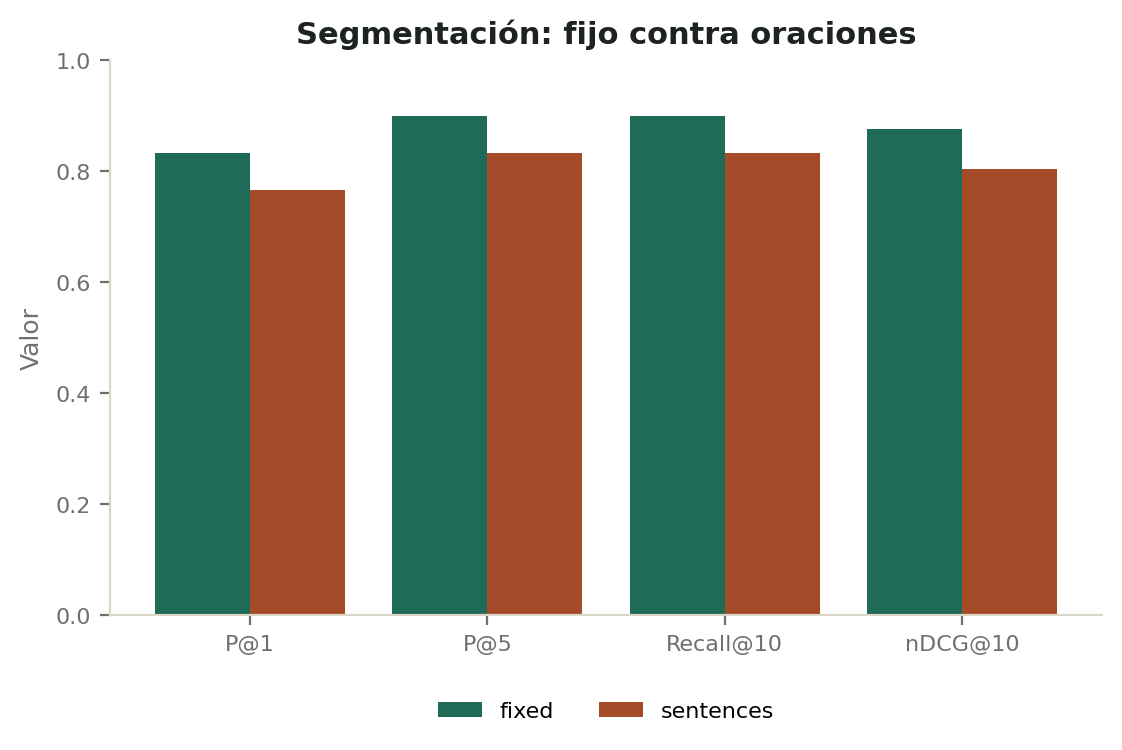
\includegraphics[width=\columnwidth]{e1_chunking.png}
\caption{Segmentaci\'on: fijo contra oraciones.}
\label{fig:e1}
\end{figure}


E2 ablacion\'o el n\'umero de fragmentos. Con el silver del piloto, el documento relevante est\'a siempre en el top-3, as\'i que $k=3$, 5 y 10 devuelven las mismas m\'etricas de calidad. La \'unica diferencia significativa es la latencia: $k=3$ tarda 1,64 ms menos que $k=10$ y $k=5$ tarda 0,94 ms menos. Se fija $k=5$ como margen para preguntas comparativas que no est\'an en el conjunto, sabiendo que el coste es m\'as contexto en generaci\'on, no m\'as latencia de recuperaci\'on.

\begin{figure}[t]
\centering
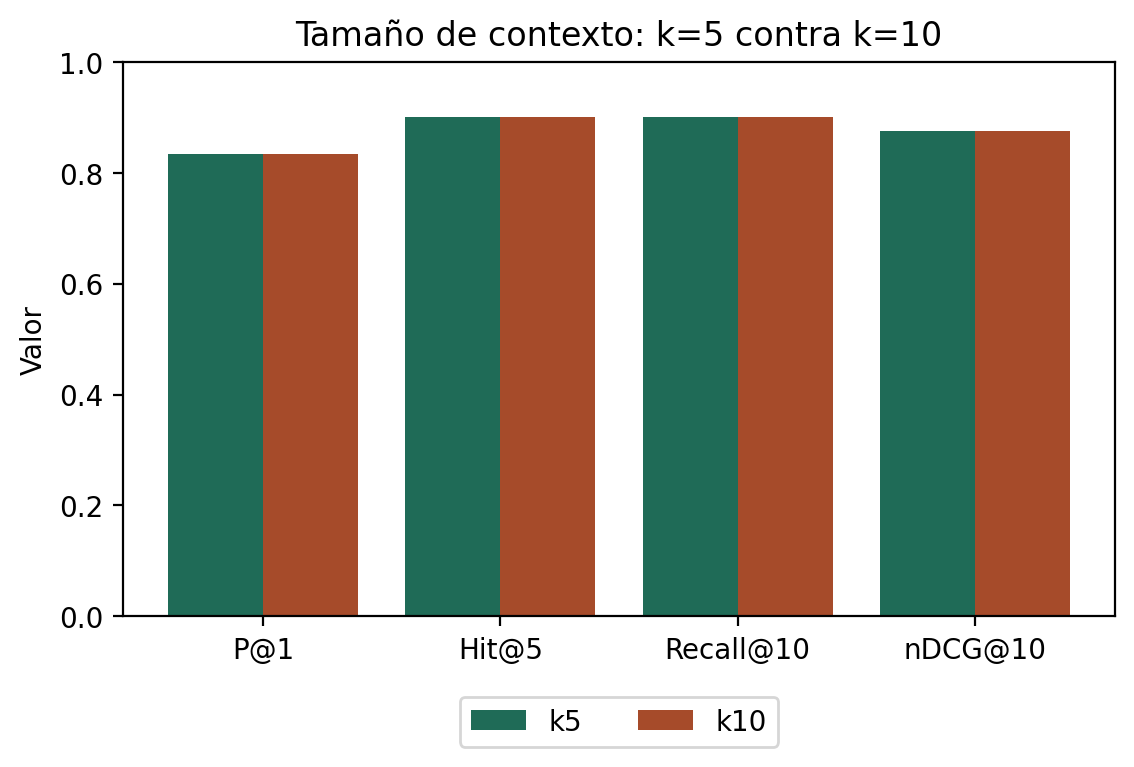
\includegraphics[width=\columnwidth]{e2_k5_vs_k10.png}
\caption{Tama\~no del contexto: $k=5$ contra $k=10$.}
\label{fig:e2}
\end{figure}


\begin{figure}[t]
\centering
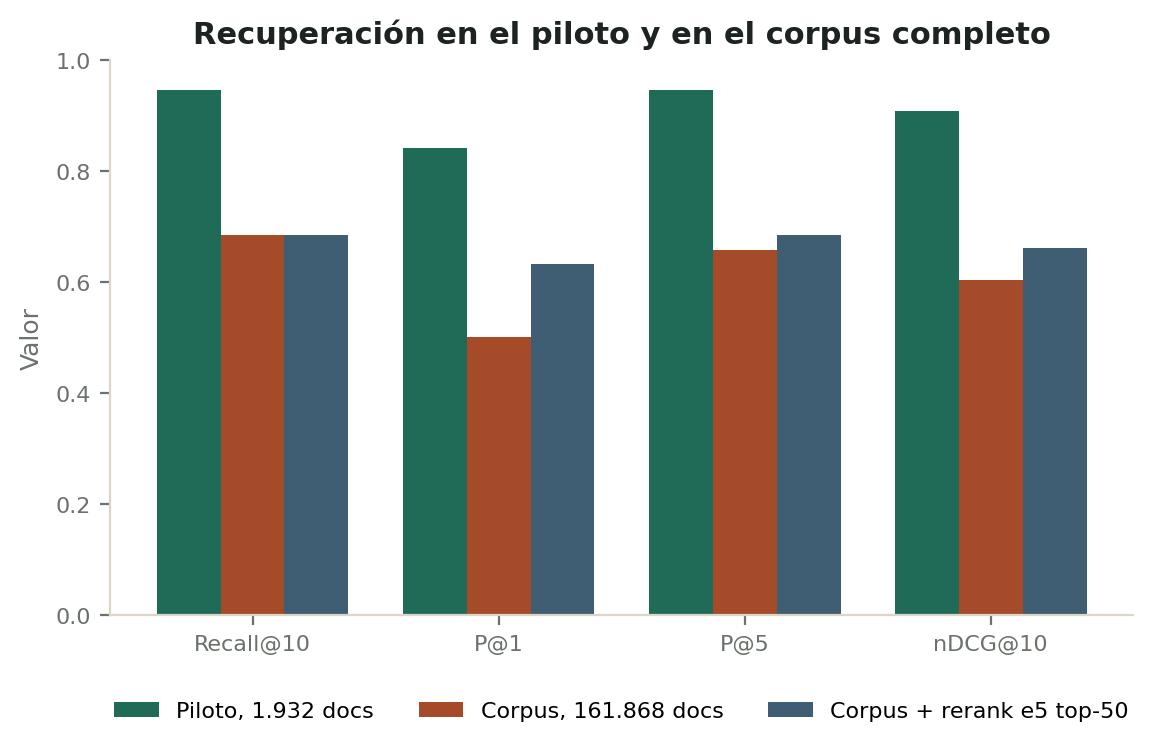
\includegraphics[width=\columnwidth]{escala_e6_e7.png}
\caption{Recuperaci\'on con e5-base sobre el silver de 38 preguntas respondibles: piloto (1.932 documentos), corpus completo (161.868 documentos) y corpus con reranker sobre el top-50. El piloto y el corpus usan \'indices separados.}
\label{fig:escala}
\end{figure}

\subsection{Codificadores y escala}

E3 compar\'o e5-base con qwen3-embedding:8b sobre el piloto, con 18 preguntas de desarrollo. qwen3 recupera mejor: Recall@10 perfecto y 6,4 puntos m\'as de nDCG. El problema es el coste. e5-base index\'o el corpus completo en 2 h 41 min medidos en la RX 9070 XT. qwen3-embedding:8b no se index\'o entero: las 23 horas son una extrapolaci\'on desde el rendimiento por lote, no un tiempo medido. Se adopta e5-base para la ingesta y qwen3 queda como comparaci\'on documentada.

E6 midi\'o el mismo pipeline sobre el corpus completo. La Figura~\ref{fig:escala} muestra la ca\'ida. La ca\'ida es el hallazgo m\'as importante del trabajo: con el mismo codificador y los mismos par\'ametros de \'indice en colecciones separadas, y las mismas 38 preguntas, Recall@10 pasa de 0,947 a 0,684 y nDCG de 0,909 a 0,594 al crecer de 1.932 a 161.868 documentos. La latencia no explica la ca\'ida (40 ms contra 42 ms). El experimento observa la ca\'ida al aumentar la escala; no separa competencia entre fragmentos, truncamiento del texto ni segmentaci\'on.

\begin{table}[t]
\centering
\footnotesize
\caption{E6: piloto contra corpus completo con e5-base (38 preguntas).}
\label{tab:e6}
\begin{tabular}{lrrrrr}
\toprule
Corpus & Recall@10 & P@1 & Hit@5 & nDCG & Span \\
\midrule
Piloto (1.932 docs) & \textbf{0,947} & \textbf{0,842} & \textbf{0,947} & \textbf{0,909} & \textbf{0,895} \\
Completo (161.868) & 0,684 & 0,474 & 0,658 & 0,594 & 0,658 \\
\bottomrule
\end{tabular}
\end{table}

E8 y E10 buscaron un recuperador mejor. BM25 sparse sube el recall a 0,763 y es ocho veces m\'as r\'apido, pero su techo de cobertura es bajo. bge-m3 llega a 0,842 de Recall@10 y 0,708 de nDCG, y recupera el ingl\'es de 0,111 a 0,667. La Tabla~\ref{tab:codificadores} resume.

\begin{table}[t]
\centering
\footnotesize
\caption{E10: recuperadores sobre el corpus completo (38 preguntas).}
\label{tab:codificadores}
\begin{tabular}{lrrrrr}
\toprule
M\'etodo & Recall@10 & P@1 & Hit@5 & nDCG & p50 \\
\midrule
Denso e5 & 0,684 & 0,500 & 0,658 & 0,604 & 48 ms \\
BM25 sparse & 0,763 & \textbf{0,684} & 0,737 & \textbf{0,727} & \textbf{7 ms} \\
bge-m3 & \textbf{0,842} & 0,553 & \textbf{0,816} & 0,708 & 56 ms \\
\bottomrule
\end{tabular}
\end{table}

E11 ajust\'o \texttt{ef} y prob\'o la fusi\'on con BM25. \texttt{ef}=800 sube el recall 2,6 puntos y el nDCG 1,3 con 6 ms m\'as. La fusi\'on 0,5/0,5 empata en recall y sube nDCG 6,9, P@1 13,2 y cobertura de span 5,3. Con el silver de un solo relevante la fusi\'on parec\'ia ganar. E12 repiti\'o la comparaci\'on con el silver ampliado: el denso recupera m\'as documentos nuevos (Recall@10 0,921 contra 0,890 y nDCG 0,827 contra 0,804). E12 se queda con la base densa, \texttt{ef}=800, sin fusi\'on; la ruta desplegada despu\'es es la uni\'on h\'ibrida, elegida sobre el conjunto de desarrollo.

\subsection{Solr como backend de recuperaci\'on}

Solr 9 se despleg\'o como un servicio m\'as del stack de Swarm, con imagen, puerto, CPU y memoria parametrizados. El \'indice replica los 618.286 fragmentos con un esquema de 13 campos y b\'usqueda \texttt{edismax} sobre \texttt{text} y \texttt{title}$^2$. La Tabla~\ref{tab:solr} compara el mismo silver de 38 preguntas. Solr con BM25 iguala el recall y el Hit@5 del BM25 de Milvus, pero pierde P@1 y nDCG. Con bge-m3, Solr alcanza 0,605 de recall, por debajo del denso de Milvus (0,842); la diferencia es consistente con el \'indice HNSW por defecto de Solr, que no se ajust\'o, y no con el embedding, que es el mismo. El backend es sustituible, pero el denso de Milvus sigue siendo la mejor opci\'on para la recuperaci\'on inicial; una comparaci\'on justa de Solr denso exige ajustar \texttt{hnswBeamWidth} y reconstruir el \'indice. El servicio se levanta con \texttt{scripts/deploy\_solr.sh} y la API de la demo corre en el puerto 8011 con \texttt{RETRIEVER=solr}.

\begin{table}[t]
\centering
\footnotesize
\setlength{\tabcolsep}{3pt}
\caption{Solr contra los recuperadores de Milvus sobre las 38 preguntas respondibles.}
\label{tab:solr}
\begin{tabular}{lrrrrr}
\toprule
Recuperador & Recall@10 & P@1 & Hit@5 & nDCG & p50 \\
\midrule
Solr BM25 & 0,763 & 0,526 & 0,737 & 0,652 & 37 ms \\
Solr bge-m3 & 0,605 & 0,395 & 0,579 & 0,510 & 109 ms \\
Milvus BM25 & 0,763 & \textbf{0,684} & 0,737 & \textbf{0,727} & \textbf{7 ms} \\
Milvus bge-m3 & \textbf{0,842} & 0,553 & \textbf{0,816} & 0,708 & 56 ms \\
\bottomrule
\end{tabular}
\end{table}

\subsection{Reordenamiento}

E7 midi\'o el cross-encoder sobre el top-50 con e5 en el corpus completo: P@1 sube de 0,474 a 0,632 y nDCG de 0,594 a 0,661, pero el Recall@10 se queda en 0,684; Hit@5 sube de 0,658 a 0,684 y la cobertura de span de 0,632 a 0,658. El coste es de 3,1 s por consulta. La mejora de orden no compensa el coste si se reordena tanto.

El denso a $k=10$ recupera 0,912 de recall y 0,818 de nDCG. Con bge-m3 se prob\'o reordenar 5 y 20 candidatos. La Tabla~\ref{tab:rerank} muestra que el top-20 baja el recall a 0,864 y el Hit@5 a 0,921, mientras que el top-5 mantiene 0,895 de recall y 0,947 de Hit@5, y sube el nDCG a 0,865 y el P@1 a 0,868 con 1,30 s. La tabla mide el reordenador en CPU; en la configuraci\'on final corre en GPU, con 0,68 s para 50 pares. La configuraci\'on final no reordena el top-5 denso: reordena la uni\'on con BM25 y recorta a 10.

\begin{table}[t]
\centering
\footnotesize
\caption{Reordenamiento con bge-m3 (38 preguntas).}
\label{tab:rerank}
\begin{tabular}{lrrrrr}
\toprule
Configuraci\'on & Recall & nDCG & P@1 & Hit@5 & p50 \\
\midrule
Denso top-5 & 0,895 & 0,809 & 0,737 & 0,947 & 0,10 s \\
Rerank top-5 & 0,895 & \textbf{0,865} & \textbf{0,868} & \textbf{0,947} & 1,30 s \\
Rerank top-20 & 0,864 & 0,853 & \textbf{0,868} & 0,921 & 5,46 s \\
\bottomrule
\end{tabular}
\end{table}


\subsection{Modelos generativos}

E4 compar\'o cuatro modelos con la misma evidencia: 19 preguntas respondibles y 5 sin respuesta, tres repeticiones, anotaci\'on humana ciega de la primera repetici\'on. La anotaci\'on cubre 18 de las 19 respondibles. La Tabla~\ref{tab:e4} muestra las medias de los dos anotadores en escala de 0 a 3. gemma2:2b gana en correcci\'on, citas y abstenci\'on. La fidelidad no se usa para el veredicto porque su acuerdo es $\kappa=0,12$. qwen2.5:1.5b es el m\'as r\'apido pero no cita en el 89,5\,\% de los casos. llama3.2:3b cita la mitad de las veces. llama3.2:1b se abstiene en el 73,7\,\% de las preguntas respondibles y no se recomienda.

\begin{table}[t]
\centering
\footnotesize
\caption{E4: anotaci\'on humana (0 a 3) y conducta autom\'atica.}
\label{tab:e4}
\begin{tabular}{lrrrr}
\toprule
Modelo & Correcci\'on & Citas & Abstenci\'on & Sin citas \\
\midrule
gemma2:2b & \textbf{2,81} & \textbf{2,67} & \textbf{2,89} & \textbf{0,0\,\%} \\
qwen2.5:1.5b & 2,31 & 0,00 & 2,81 & 89,5\,\% \\
llama3.2:3b & 2,22 & 0,86 & 2,69 & 56,1\,\% \\
llama3.2:1b & 0,42 & 0,28 & 1,61 & 15,8\,\% \\
\bottomrule
\end{tabular}
\end{table}

La hip\'otesis H1, que esperaba que llama3.2:3b superara a los dem\'as en correcci\'on y citas, se refuta. La evidencia recuperada es la misma entre modelos; lo que cambia es el generador. La comparaci\'on fij\'o la familia de modelos peque\~nos. El generador final es gemma4:e4b, que no estaba en E4: se adopt\'o despu\'es por contexto largo y MTP, no por ganar una comparaci\'on directa, y se valid\'o en la corrida final.

Se prob\'o un generador local de 27B (\texttt{qwen3.8:docs-32k-q3\_k\_s}, Q3) con el mismo pipeline y el mismo prompt. En test obtiene 0,917 de exactitud, 0,489 de cobertura, 0,657 de correcci\'on RAGAS y 10,3 s de mediana, frente a 0,917, 0,522, 0,652 y 1,2 s del 4B. El modelo grande no mejora de forma apreciable las m\'etricas y multiplica la latencia por ocho; el 4B se queda como generador desplegado.

\subsection{Inyecci\'on de instrucciones}

E5 insert\'o instrucciones expl\'icitas en cinco documentos sint\'eticos por modelo. Es una prueba exploratoria: no cubre el generador final ni demuestra robustez general. Dos de los tres modelos las ignoraron. gemma2:2b obedeci\'o una de cinco y a\~nadi\'o la palabra pedida a una respuesta por lo dem\'as correcta. La regla de dise\~no que sale de aqu\'i es que el prompt debe delimitar la evidencia y ordenar expl\'icitamente ignorar instrucciones internas, y esa orden debe repetirse despu\'es del bloque de contexto.

\begin{table}[t]
\centering
\footnotesize
\caption{E5: instrucciones inyectadas en el texto recuperado.}
\label{tab:e5}
\begin{tabular}{lrrr}
\toprule
Modelo & Obedeci\'o & Respondi\'o el hecho & Se abstuvo \\
\midrule
gemma2:2b & 1/5 & 4/5 & 0/5 \\
llama3.2:3b & 0/5 & 5/5 & 0/5 \\
qwen2.5:1.5b & 0/5 & 5/5 & 0/5 \\
\bottomrule
\end{tabular}
\end{table}


\subsection{Prompts y mejoras rechazadas}

La fase 6 prob\'o cuatro mejoras sobre la configuraci\'on de referencia y la fase 7 prob\'o diversidad. La referencia de estas fases era el top-5 denso con reranker; la uni\'on con BM25 se adopt\'o despu\'es, en el conjunto reservado. Ninguna de las variantes de las fases 6 y 7 supera a esa referencia. La Tabla~\ref{tab:fases} resume. El filtro por score pierde recall; reordenar el top-20 pierde Hit@5 y multiplica la latencia; la expansi\'on de consulta baja el recall y el nDCG; el prompt v4 no mejora la cobertura de tokens; y MMR baja el recall 8 puntos. El prompt v4 entreg\'o 37 de 38 y 25 de 37 de cobertura de tokens, sin mejora. Todas se rechazan y la configuraci\'on se mantiene.

\begin{table*}[t]
\centering
\footnotesize
\caption{Fases 6 y 7: variantes probadas sobre 38 preguntas. La referencia es el top-5 con reranker.}
\label{tab:fases}
\begin{tabular}{lrrrrl}
\toprule
Variante & Recall & nDCG & P@1 & Hit@5 & Decisi\'on \\
\midrule
Top-5 con reranker & \textbf{0,895} & \textbf{0,865} & \textbf{0,868} & \textbf{0,947} & Referencia \\
Rerank top-20 & 0,864 & 0,853 & \textbf{0,868} & 0,921 & Rechazada \\
Filtro por score 0,8 & 0,838 & 0,837 & \textbf{0,868} & 0,921 & Rechazada \\
Filtro por score 0,9 & 0,825 & 0,830 & \textbf{0,868} & 0,921 & Rechazada \\
Expansi\'on de consulta & 0,825 & 0,739 & 0,658 & 0,895 & Rechazada \\
MMR coseno 0,5 & 0,868 & 0,784 & 0,737 & \textbf{0,947} & Rechazada \\
MMR con reranker 0,7 & 0,816 & 0,818 & \textbf{0,868} & 0,921 & Rechazada \\
\bottomrule
\end{tabular}
\end{table*}


\subsection{Compuerta de dominio}

La compuerta se entren\'o con 160 preguntas: 60 de dominio y 100 de fuera, con 103 de train, 37 de dev y 20 de test. Los 40 negativos nuevos son entidades inventadas, eventos futuros y conocimiento general. La Tabla~\ref{tab:compuerta} muestra el resultado en el test interno y en el conjunto reservado. En test el F1 es 0,952, con 0 falsos aceptados de 9 y 1 falso rechazo de 11. En el conjunto reservado, con 20 directas y 5 negativas, el F1 es 0,919: rechaza las 5 negativas y 3 de las 20 directas. El umbral es 0,4, elegido por validaci\'on cruzada. Con 5 negativas, el 0/5 no demuestra una tasa nula de falsos aceptados en uso general; solo acota el intervalo observado.

\begin{table}[t]
\centering
\footnotesize
\caption{Compuerta de dominio: test interno y conjunto reservado.}
\label{tab:compuerta}
\begin{tabular}{lrrrrrr}
\toprule
Split & $n$ & Dominio & Fuera & Precisi\'on & Recall & F1 \\
\midrule
Test & 20 & 11 & 9 & 1,000 & 0,909 & 0,952 \\
Reservado & 25 & 20 & 5 & 1,000 & 0,850 & 0,919 \\
\bottomrule
\end{tabular}
\end{table}

\subsection{RAGAS}

La Tabla~\ref{tab:ragas} compara cuatro configuraciones. El h\'ibrido es la ruta desplegada: uni\'on densa y BM25, $k=10$ y sin compuerta. El denso $k=10$ comparte $k$ con el h\'ibrido, as\'i que su diferencia a\'isla el recuperador: el h\'ibrido gana relevancia, precisi\'on y correcci\'on, y pierde fidelidad, con la misma cobertura. El denso $k=5$, con menos contexto, gana fidelidad, relevancia, precisi\'on y correcci\'on, y pierde cobertura: el efecto de $k$ es mayor que el del recuperador. La \'ultima columna cambia juez y embeddings, as\'i que es observacional. Las diferencias entre las tres primeras son descriptivas.

\begin{table*}[t]
\centering
\footnotesize
\caption{RAGAS: h\'ibrido, denso con $k=10$, denso con $k=5$ y configuraci\'on anterior, con $n$ entre par\'entesis. Las tres primeras usan juez gemma4:e4b y embeddings bge-m3; la \'ultima cambia juez y embeddings, as\'i que su comparaci\'on es observacional.}
\label{tab:ragas}
\begin{tabular}{lrrrr}
\toprule
M\'etrica & H\'ibrido $k=10$ & Denso $k=10$ & Denso $k=5$ & Anterior \\
\midrule
Fidelidad & 0,920 (38) & 0,932 (38) & \textbf{0,952} (38) & 0,925 (36) \\
Relevancia & 0,788 (38) & 0,765 (38) & \textbf{0,840} (38) & 0,798 (38) \\
Precisi\'on del contexto & 0,867 (36) & 0,810 (36) & \textbf{0,881} (34) & 0,760 (36) \\
Cobertura del contexto & \textbf{0,947} (38) & \textbf{0,947} (38) & 0,921 (38) & 0,842 (38) \\
Correcci\'on & 0,607 (38) & 0,569 (38) & \textbf{0,657} (38) & 0,705 (37) \\
\bottomrule
\end{tabular}
\end{table*}

\subsection{Latencia y MTP}

La Tabla~\ref{tab:mtp} muestra el efecto del draft. El draft 3 es el m\'as r\'apido: 217,1 tokens por segundo frente a 193,5 con 5 y 159,5 con 7. La decodificaci\'on especulativa es exacta: el draft propone y el modelo objetivo verifica, as\'i que la salida no cambia.

\begin{table}[t]
\centering
\footnotesize
\caption{MTP: tokens por segundo seg\'un el draft.}
\label{tab:mtp}
\begin{tabular}{lr}
\toprule
Draft & Tokens/s \\
\midrule
3 & \textbf{217,1} \\
5 & 193,5 \\
7 & 159,5 \\
\bottomrule
\end{tabular}
\end{table}

La corrida de referencia de la configuraci\'on anterior (densa y reranker en CPU) es la del 2 de noviembre, con el c\'odigo del commit \texttt{125bbc7}: 7.938 ms sin razonamiento y 6.834 ms con razonamiento; los CSV est\'an en \texttt{reports/tablas/}. El reranker en CPU aporta 1,30 s de mediana. Con la configuraci\'on final (uni\'on h\'ibrida y reranker en GPU), el conjunto reservado dio 6.154 ms de media (mediana 5.578, p95 9.136) sobre 25 preguntas. La compuerta reutiliza la puntuaci\'on del reranker, as\'i que no a\~nade una segunda pasada.

\subsection{Observabilidad y evaluaci\'on continua}
\label{sec:observabilidad}

Cada consulta deja una traza en Langfuse 4.78, desplegado en el servidor como un servicio m\'as del stack. La traza \texttt{ask} contiene los spans \texttt{retrieve}, \texttt{rerank}, \texttt{generate} y \texttt{grounding}, con los fragmentos recuperados, el prompt, la respuesta, las citas, los tokens y las latencias. Los scores \texttt{citation\_valid}, \texttt{grounded} y \texttt{latency\_ms} se calculan en la misma petici\'on, y el identificador de la traza se devuelve en la respuesta para enlazarla con la corrida de evaluaci\'on. La Figura~\ref{fig:trace} muestra la traza de una consulta real.

\begin{figure*}[t]
\centering
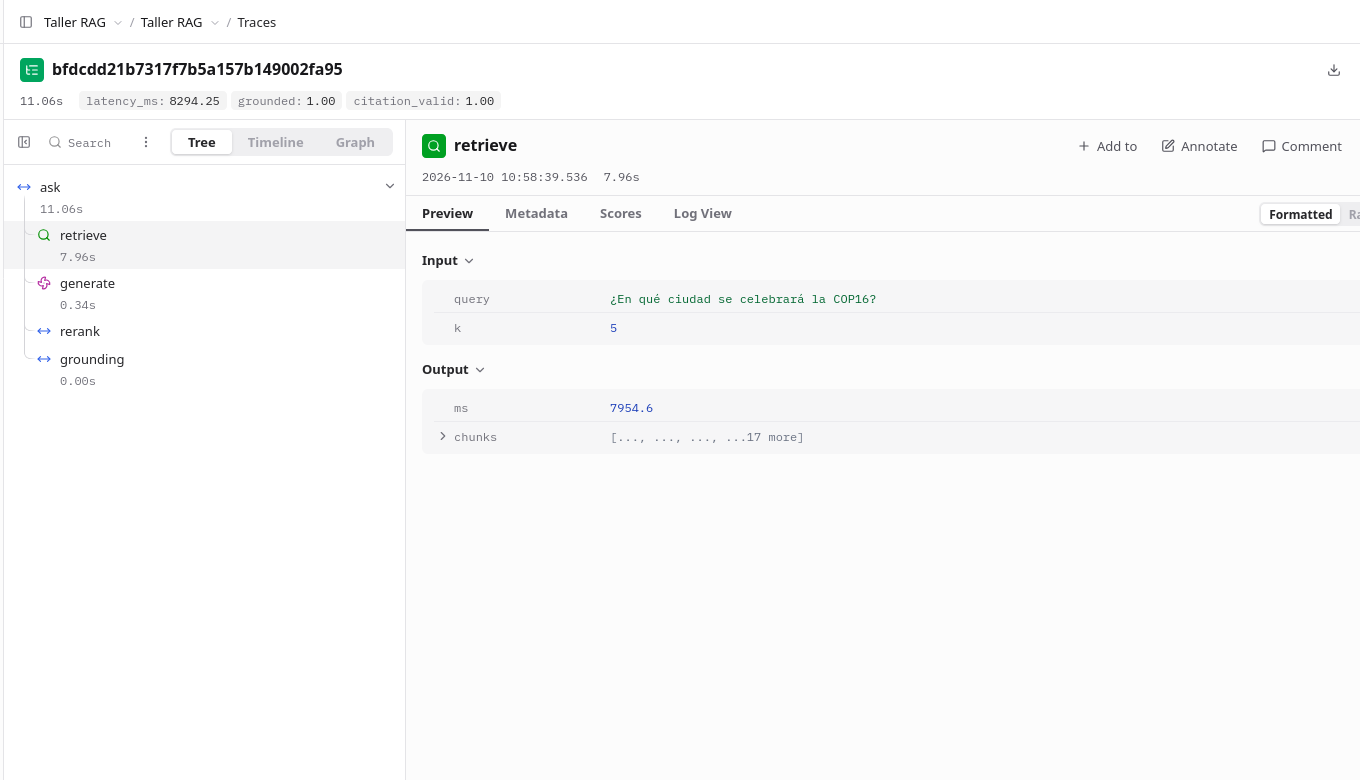
\includegraphics[width=\textwidth]{langfuse_trace_crop.png}
\caption{Traza de una consulta en Langfuse: spans de recuperaci\'on, reordenamiento, generaci\'on y anclaje, con los scores de la petici\'on.}
\label{fig:trace}
\end{figure*}

El conjunto dorado vive como Dataset de Langfuse. Cada corrida es un experimento que enfrenta la respuesta esperada con la respuesta del modelo y calcula cuatro scores por \'item: \texttt{correct}, \texttt{token\_recall}, \texttt{citation\_valid} y \texttt{grounded}. La Figura~\ref{fig:langfuse} muestra la vista de evaluaci\'on con la pregunta, el gold, los scores y la respuesta. La Tabla~\ref{tab:observabilidad} resume las tres corridas sobre las 43 preguntas del silver.

\begin{figure*}[t]
\centering
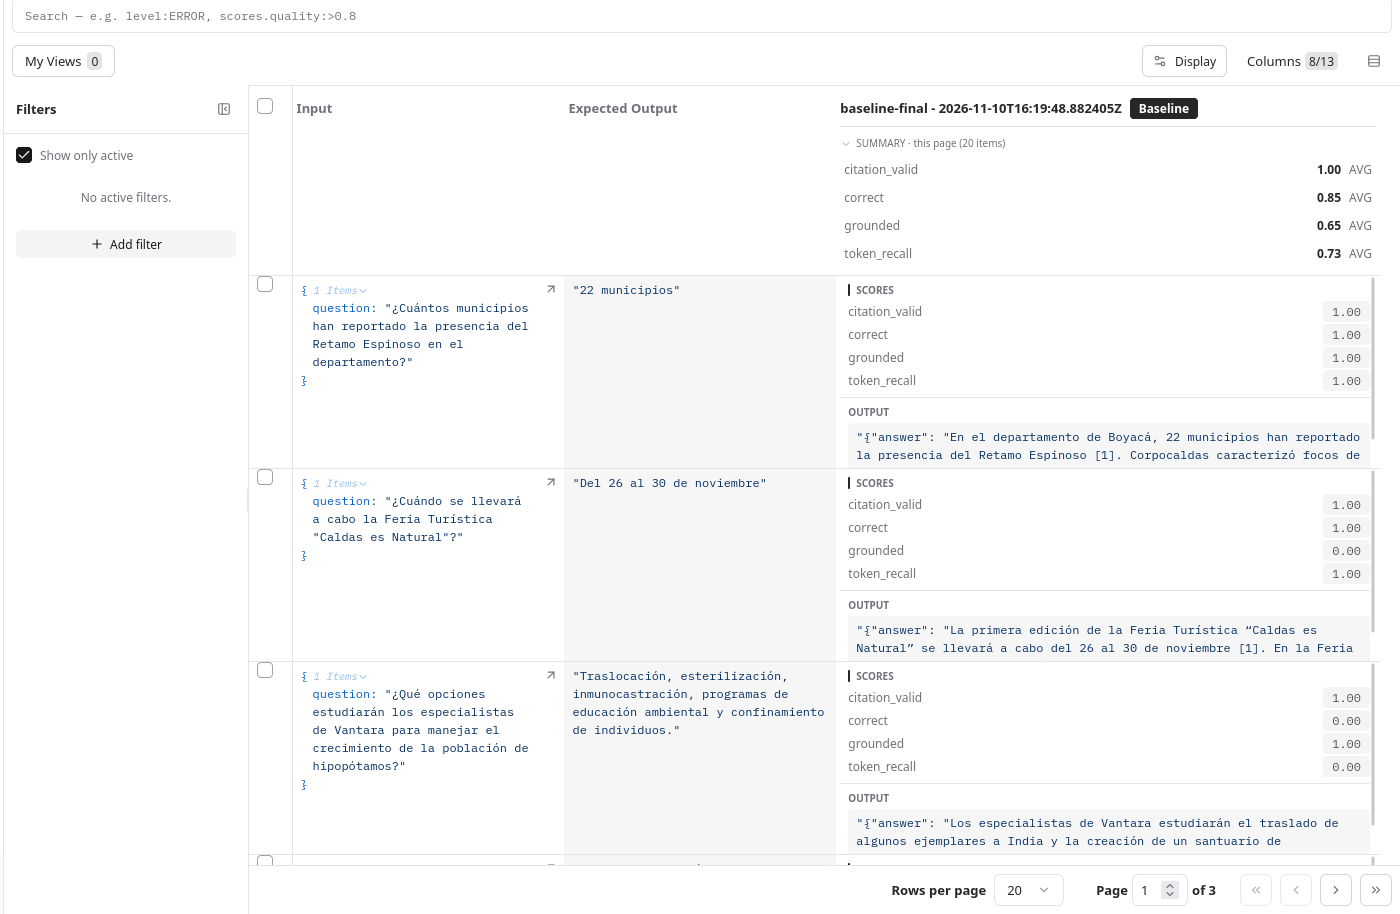
\includegraphics[width=\textwidth]{langfuse_experiment_crop.png}
\caption{Experimento en Langfuse: pregunta, respuesta esperada, scores y respuesta del modelo, con la comparaci\'on por \'item.}
\label{fig:langfuse}
\end{figure*}

\begin{table}[t]
\centering
\footnotesize
\caption{Corridas registradas en Langfuse sobre las 43 preguntas del silver. La exactitud incluye las 5 preguntas sin respuesta.}
\label{tab:observabilidad}
\begin{tabular}{lrrrr}
\toprule
Corrida & Exactitud & Cobertura & Anclaje & p50 \\
\midrule
Uni\'on h\'ibrida & 0,837 & 0,626 & 0,744 & 0,42 s \\
Grafo h\'ibrido & \textbf{0,861} & 0,635 & 0,767 & 1,44 s \\
H\'ibrido + boost & \textbf{0,861} & \textbf{0,655} & \textbf{0,791} & 1,30 s \\
\bottomrule
\end{tabular}
\end{table}

La tabla muestra el efecto de la observabilidad: las tres corridas usan el mismo conjunto, el mismo modelo y la misma temperatura, as\'i que la diferencia es del recuperador. El registro no cambia la respuesta; cambia la capacidad de atribuirla. Sin \'el, una mejora de dos puntos en exactitud no se puede separar de la variaci\'on del muestreo ni del orden de las preguntas.

\subsection{GraphRAG ligero}
\label{sec:graphrag}

Se construy\'o un grafo de documentos y entidades en Neo4j 5.26. Cada documento se conecta con las entidades nombradas que menciona; la extracci\'on corre con spaCy en espa\~nol e ingl\'es sobre el t\'itulo y los primeros 1.500 caracteres. El grafo tiene 169.248 documentos, 248.869 entidades y 926.923 menciones, y se construye en 2.000 s en un solo proceso. La Figura~\ref{fig:neo4j} muestra un documento y sus entidades.

\begin{figure}[t]
\centering
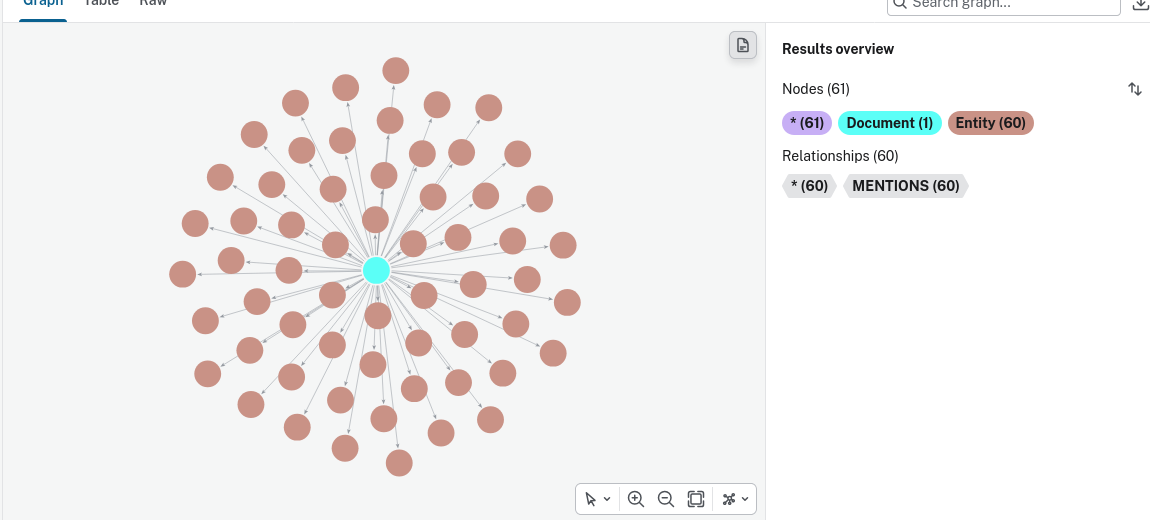
\includegraphics[width=\columnwidth]{neo4j_graph_crop.png}
\caption{Grafo en Neo4j: un documento y las entidades que menciona.}
\label{fig:neo4j}
\end{figure}

Se probaron dos formas de usar el grafo. \texttt{graph\_hybrid} fusiona los candidatos del grafo con la uni\'on densa y BM25 antes del reordenamiento. \texttt{hybrid\_boost} deja intacta la recuperaci\'on y suma al \texttt{rerank\_score} un bono por cada entidad de la consulta presente en el fragmento. La Tabla~\ref{tab:graphrag} compara ambos modos con el baseline en las 43 preguntas y en un conjunto nuevo de 10 preguntas multi-documento.

\begin{table*}[t]
\centering
\footnotesize
\caption{GraphRAG contra la uni\'on h\'ibrida. Exactitud y cobertura de tokens sobre las 43 preguntas del silver y sobre 10 preguntas multi-documento.}
\label{tab:graphrag}
\begin{tabular}{lrrrr}
\toprule
Modo & Exactitud (43) & Cobertura (43) & Exactitud (10) & Cobertura (10) \\
\midrule
Uni\'on h\'ibrida & 0,837 & 0,626 & \textbf{0,900} & 0,878 \\
Grafo h\'ibrido & \textbf{0,861} & 0,635 & 0,700 & 0,694 \\
H\'ibrido + boost & \textbf{0,861} & \textbf{0,655} & \textbf{0,900} & \textbf{0,889} \\
\bottomrule
\end{tabular}
\end{table*}

El resultado separa dos usos que suelen confundirse. El grafo como fuente de candidatos mejora una pregunta en el silver, pero pierde 20 puntos en el conjunto multi-documento: el reordenador prefiere documentos que el grafo trae por entidades ruidosas y desplaza fragmentos que la recuperaci\'on densa ya ten\'ia. El grafo como reordenador, en cambio, sube la cobertura de tokens y el anclaje en ambos conjuntos sin degradar la exactitud. La diferencia es consistente con la calidad de la extracci\'on: las claves no pasan por un enlace de entidades y muchas son frases largas, as\'i que el grafo sirve para desempatar, no para sustituir al \'indice. GraphRAG no es una mejora gratuita; con este corpus y este extractor, el uso defendible es el boost. Se reconstruy\'o el grafo con un filtro de entidades (m\'aximo 4 tokens, sin d\'igitos iniciales, MISC de m\'aximo 3): qued\'o en 206.614 entidades y 852.751 menciones. Con ese grafo y el prompt v3, \texttt{graph\_hybrid} obtiene 0,875 en test y 0,880 en el reservado, mientras el boost obtiene 0,917 y 0,840; en las 10 preguntas multi-documento el grafo sigue en 0,700. La limpieza mejora la precisi\'on del grafo en el reservado, pero no revierte la p\'erdida multi-documento.

\subsection{Mejora de la respuesta y evaluaci\'on sem\'antica}
\label{sec:prompt-v3}

El an\'alisis de errores mostr\'o que la recuperaci\'on no era el \'unico cuello de botella: RAGAS daba 0,947 de cobertura de contexto y 0,607 de correcci\'on. El contexto tra\'ia la evidencia, pero el modelo omit\'ia datos en las preguntas de lista o de dos partes. Se prob\'o un prompt v3 que pide la respuesta directa, todos los datos pedidos y la lista completa, con dos ejemplos y un l\'imite de tres frases. La Tabla~\ref{tab:prompt} compara el prompt v2 y el v3 con el mismo recuperador (uni\'on h\'ibrida m\'as el boost del grafo) en test (24 preguntas) y en el reservado (25).

\begin{table*}[t]
\centering
\footnotesize
\caption{Prompt v2 contra prompt v3 con el mismo recuperador. Exactitud y cobertura de tokens sobre test (24) y el reservado (25).}
\label{tab:prompt}
\begin{tabular}{lrrrr}
\toprule
Configuraci\'on & Exactitud test & Cobertura test & Exactitud reservado & Cobertura reservado \\
\midrule
v2 + boost & \textbf{0,917} & \textbf{0,541} & \textbf{0,840} & \textbf{0,440} \\
v3 + boost & \textbf{0,917} & 0,522 & \textbf{0,840} & \textbf{0,440} \\
v3 sin boost & 0,875 & 0,486 & \textbf{0,840} & \textbf{0,440} \\
\bottomrule
\end{tabular}
\end{table*}

La exactitud es la misma: 0,917 en test y 0,840 en el reservado. La diferencia aparece en la evaluaci\'on sem\'antica. La Tabla~\ref{tab:ragas-v3} repite RAGAS sobre las 19 preguntas respondibles de test y las 20 del reservado. El prompt v3 sube la correcci\'on de 0,590 a 0,652 con el mismo recuperador y la misma exactitud; sin el boost llega a 0,687, a costa de una pregunta exacta. La diferencia pareada es +0,062, IC 95\,\% $[-0{,}019, 0{,}145]$, $p=0{,}14$: con 19 preguntas es una tendencia, no un resultado concluyente. La exactitud no cambia (diferencia 0, IC $[0, 0]$). La fidelidad queda en 1,0 y la cobertura de contexto en 1,0: el generador no inventa y la evidencia alcanza.

\begin{table*}[t]
\centering
\footnotesize
\caption{RAGAS con prompt v2 y v3. Test: 19 preguntas respondibles. Reservado: 20. Juez gemma2:2b y embeddings qwen3-embedding:8b.}
\label{tab:ragas-v3}
\begin{tabular}{lrrrrr}
\toprule
Configuraci\'on & Fidelidad & Relevancia & Precisi\'on & Cobertura & Correcci\'on \\
\midrule
v2 + boost (test) & \textbf{1,000} & \textbf{0,790} & 0,735 & \textbf{1,000} & 0,590 \\
v3 + boost (test) & \textbf{1,000} & 0,772 & 0,728 & \textbf{1,000} & 0,652 \\
v3 + boost (reservado) & 0,938 & 0,798 & 0,808 & \textbf{1,000} & 0,629 \\
v3 sin boost (test) & \textbf{1,000} & 0,799 & \textbf{0,751} & \textbf{1,000} & \textbf{0,687} \\
v3 sin boost (reservado) & 0,975 & \textbf{0,856} & \textbf{0,863} & \textbf{1,000} & 0,655 \\
\bottomrule
\end{tabular}
\end{table*}

La m\'etrica l\'exica subestima las respuestas correctas cuando cambian de idioma. En el reservado, r-012 responde \textit{Foro Econ\'omico Mundial} por \textit{World Economic Forum} y r-019 responde \textit{avispa asi\'atica} por \textit{Asian Hornet}; ambas son correctas y el chequeo de contenci\'on las marca como fallo, mientras RAGAS las punt\'ua por encima de 0,7. Con esa correcci\'on, el reservado pasa de 21 a 23 aciertos sobre 25. La configuraci\'on final es v3 con el boost del grafo: 0,917 de exactitud en test, 0,840 en el reservado, 0,652 de correcci\'on RAGAS en test y 0,629 en el reservado, con 0,938 de fidelidad. El boost no cambia la exactitud del reservado y su efecto en la correcci\'on es +0,030 en test (IC $[-0{,}007, 0{,}074]$, $p=0{,}14$) y +0,010 en el reservado (IC $[-0{,}027, 0{,}065]$, $p=0{,}75$); ninguna de las dos excluye cero. Si se prioriza la correcci\'on sem\'antica sobre una pregunta exacta, v3 sin boost es la mejor opci\'on: 0,687 en test y 0,655 en el reservado, tambi\'en sin diferencia concluyente.

\subsection{Resumen de resultados}

La Figura~\ref{fig:resumen} re\'une los tres resultados principales: RAGAS por configuraci\'on, las pol\'iticas de ambig\"uedad sobre el silver humano y el flujo del conjunto reservado con y sin compuerta.

\begin{figure*}[t]
\centering
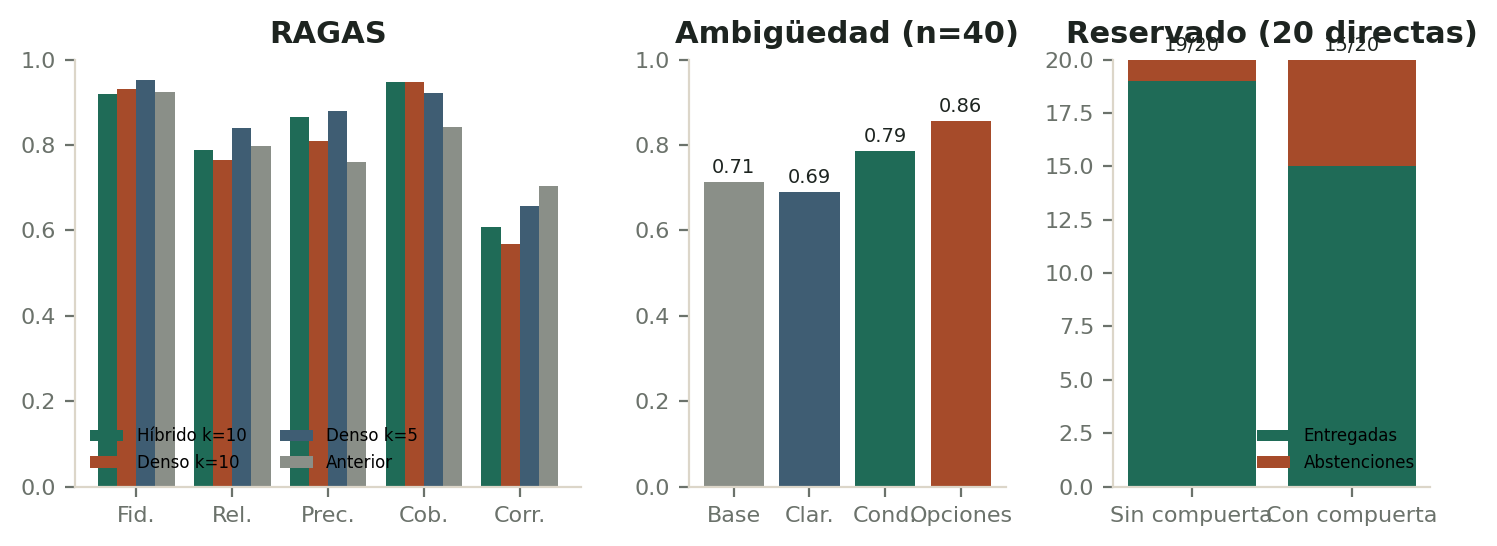
\includegraphics[width=\textwidth]{resumen_final.png}
\caption{Resumen de resultados: RAGAS por configuraci\'on, pol\'iticas de ambig\"uedad y flujo del conjunto reservado con y sin compuerta.}
\label{fig:resumen}
\end{figure*}

\subsection{Conjunto reservado}
\label{sec:reservado}

El silver exploratorio se us\'o para elegir la configuraci\'on densa, as\'i que no mide generalizaci\'on. Se construy\'o un conjunto reservado de 25 preguntas: 20 directas y 5 sin respuesta, 15 en espa\~nol y 10 en ingl\'es, 14 de prensa y 6 de Bluesky. Las preguntas se generaron con Gemma4 y se validaron autom\'aticamente; no son una muestra humana independiente. El conjunto se congel\'o antes de evaluar la compuerta y se us\'o para esa evaluaci\'on. Despu\'es se us\'o tambi\'en para elegir la recuperaci\'on h\'ibrida. Por eso las m\'etricas de recuperaci\'on y respuesta de esta secci\'on son de desarrollo. La compuerta se midi\'o antes de esa elecci\'on, pero el mismo conjunto se us\'o despu\'es para elegir el h\'ibrido: sus cifras tambi\'en son de desarrollo. Una prueba independiente de la recuperaci\'on exige un conjunto nuevo. La Tabla~\ref{tab:reservado} muestra el resultado.

\begin{table}[t]
\centering
\footnotesize
\caption{Conjunto reservado: 20 preguntas directas y 5 sin respuesta, congelado antes de ejecutar; la compuerta se evalu\'o antes de elegir el h\'ibrido.}
\label{tab:reservado}
\begin{tabular}{lrr}
\toprule
M\'etrica & Valor & Denominador \\
\midrule
Recall@10 & 0,700 & 20 \\
nDCG@10 & 0,612 & 20 \\
P@1 & 0,500 & 20 \\
Hit@5 & 0,650 & 20 \\
Cobertura de span & 0,700 & 20 \\
Entregadas & 19 & 20 \\
Abstenciones en directas & 1 & 20 \\
Cobertura de tokens, entregadas & 17 & 19 \\
Cobertura de tokens, todas & 17 & 20 \\
Con cita & 1,000 & 19 \\
Abstenciones en sin respuesta & 5 & 5 \\
Compuerta rechaza & 5 & 5 \\
Latencia media & 6,2 s & 25 \\
Entregadas con compuerta (strict) & 15 & 20 \\
Cobertura de tokens con compuerta & 13 & 15 \\
Rechazos de compuerta & 3 & 20 \\
Rechazos del juez & 2 & 20 \\
\bottomrule
\end{tabular}
\end{table}


Las m\'etricas de respuesta se midieron sin la compuerta estricta; las predicciones de la compuerta se calcularon en una pasada aparte. Con la compuerta activa (\texttt{strict=True}), el flujo conjunto entrega 15 de 20 directas y se abstiene en las 5 negativas: tres directas se rechazan por dominio (r-011, r-012 y r-014) y dos por el juez de evidencia (r-005 y r-006). La cobertura de tokens de las 15 entregadas es 13/15 (0,867). La diferencia con las 19 entregas sin compuerta es el coste del filtro. El recall@10 es 0,700 y el nDCG 0,612, por debajo del 0,912 y 0,818 del silver exploratorio, pero por encima del 0,600 y 0,477 de la recuperaci\'on densa. La uni\'on con BM25 recupera r-012 y r-014, que el denso dejaba fuera, y conserva los aciertos del denso en r-009 y r-013. Seis de las 20 preguntas no recuperan el documento de referencia en el top-10; cuatro se responden correctamente con otro documento que contiene el mismo dato (r-005, r-008, r-017, r-019), una termina en abstenci\'on (r-006) y una es ambigua (r-016). El recall con un solo documento de referencia subestima la recuperaci\'on \'util: la mitad de los fallos de recall no son fallos de respuesta. La profundidad de la uni\'on no es monot\'onica: 20/20 y 30/30 suben el recall@10 a 0,750; 50/50 lo sube a 0,850 y recupera r-006, pero baja las entregas a 18 de 20 y la cobertura de tokens a 16 de 20, porque desplaza evidencia que el modelo usaba bien en r-009 y r-012. La configuraci\'on se queda en 10/20.

La cobertura de tokens entre las entregadas es 17 de 19 (89,5\,\%), y sobre las 20 directas, 17 de 20 (85\,\%). La diferencia con la recuperaci\'on densa est\'a en la uni\'on: recupera las entidades que el denso no trae. En ingl\'es el recall es 0,875 y el nDCG 0,829; en espa\~nol, 0,583 y 0,468. El ingl\'es recupera mejor, al contrario de lo que suger\'ia el silver exploratorio.

Las cinco preguntas sin respuesta se rechazan por la compuerta. En las 20 directas, la compuerta rechaza 3: r-011, r-012 y r-014. r-012 y r-014 son preguntas que la recuperaci\'on h\'ibrida s\'i puede responder, pero la compuerta solo ve el top-5 denso; es una deuda de dise\~no, no un fallo de recuperaci\'on. r-011 s\'i recupera el documento y es un falso rechazo del clasificador. La compuerta nueva baja los falsos rechazos de 6 a 3 y los falsos aceptados de 1 a 0 respecto de la anterior. El 0/9 del conjunto anterior no se confirma como tasa nula, pero el 0/5 tampoco la demuestra.

El fallo m\'as grave es r-006: la pregunta pide los 95 votos en la C\'amara de Representantes y el sistema se abstiene. La evidencia recuperada no contiene la cifra correcta en el top-10, y el modelo prefiere no responder. r-016 es una pregunta ambigua del propio conjunto: no nombra el concierto y el corpus tiene varios; se mantiene en las m\'etricas y se reporta como l\'imite de construcci\'on. r-012 entrega una respuesta evasiva: la evidencia contiene la organizaci\'on, pero el modelo enumera varias iniciativas en lugar de responder World Economic Forum. Es un fallo de generaci\'on, no de recuperaci\'on.

La latencia media del conjunto reservado es 6,2 s (mediana 5,6, p95 9,1), inferior a los 10,8 s de la corrida densa. La uni\'on y el reordenador en GPU compensan el mayor n\'umero de candidatos.

La Tabla~\ref{tab:progresion} resume la progresi\'on de la configuraci\'on. Cada fila es una decisi\'on tomada con una medici\'on, no una preferencia.

\begin{table*}[t]
\centering
\footnotesize
\caption{Progresi\'on de la configuraci\'on y m\'etrica que la justific\'o.}
\label{tab:progresion}
\begin{tabular}{lllll}
\toprule
Etapa & Cambio & Silver & M\'etrica & Decisi\'on \\
\midrule
Piloto & e5-base, 1.932 docs & piloto (38) & Recall@10 0,947 & Punto de partida \\
Escala & corpus completo & 38 & Recall@10 0,684 & El piloto sobreestima \\
Dispersa & BM25 & 38 & Recall@10 0,763 & No alcanza el techo \\
Codificador & bge-m3 & 38 & Recall@10 0,842 & Adoptado \\
\'Indice & \texttt{ef}=800 & 38 & Recall@10 0,895 & Adoptado \\
Fusi\'on & h\'ibrido RRF & 38 & Recall@10 0,895 & Empata, se descarta \\
Fusi\'on & h\'ibrido RRF & ampliado & Recall@10 0,890 & Rechazado \\
Reordenamiento & uni\'on densa+BM25 & reservado (20) & Recall@10 0,700 & Adoptado; recupera parte de la ca\'ida \\
Contexto & $k=10$ & reservado (20) & 19/20 entregadas & Adoptado \\
Prompt & v2 & 38 & 37/38 y cobertura 25/37 & Adoptado \\
Compuerta & 160 preguntas & 20 test & 0 falsos aceptados & Adoptado \\
Fase 6 & cuatro variantes & 38 & sin mejora & Rechazadas \\
Fase 7 & MMR & 38 & recall 0,816 & Rechazado \\
Compuerta & 5 negativas & reservado (5) & 5/5 rechazadas & 3/20 falsos rechazos \\
Prompt & v3 + boost & test (24) & Exactitud 0,917 & Adoptado \\
\bottomrule
\end{tabular}
\end{table*}


\section{An\'alisis de errores}
\label{sec:errores}

\subsection{Errores de recuperaci\'on}

Queda un fallo claro en el silver standard. g-031 pregunta por el municipio de gran extensi\'on y tradici\'on agropecuaria del sur del Tolima. En E6/E7 quedaba en el puesto 11 del top-50 denso; la ruta h\'ibrida lo recupera en el puesto 1 y responde Chaparral. g-046, sobre la protesta de Extinction Rebellion, no aparece ni en la uni\'on ni tras el reranker; el problema est\'a en la consulta o en el \'indice. El an\'alisis de E6/E7 se conserva como hist\'orico.

\subsection{Errores de generaci\'on}

Los modelos peque\~nos fallan de formas distintas con la misma evidencia. qwen2.5:1.5b responde sin citar en el 89,5\,\% de los casos: la respuesta puede ser correcta, pero el usuario no puede verificar de d\'onde sale. llama3.2:3b cita la mitad de las veces. llama3.2:1b se abstiene en el 73,7\,\% de las preguntas respondibles. gemma2:2b cita siempre y responde casi siempre, pero responde preguntas sin respuesta en 3 de 15 repeticiones, es decir, alucina con evidencia insuficiente. El generador final, gemma4:e4b, no estaba en esa comparaci\'on; los guardarra\'iles de cita, entidades y juez cubren parte de ese riesgo, y la compuerta lo cubre antes de generar.

\subsection{Abstenci\'on y compuerta}

La abstenci\'on tiene dos caminos. El primero ocurre antes de generar, cuando la compuerta rechaza la pregunta; el segundo, despu\'es, cuando los guardarra\'iles o el juez no encuentran respaldo. El primer camino es barato (decenas de milisegundos) y ahora rechaza las 5 preguntas sin respuesta con 0,293 a 0,436. El segundo cuesta una generaci\'on completa. La compuerta v2, con umbral 0,4, rechaza 3 de las 20 directas del reservado: r-011 es un falso rechazo del clasificador y r-012/r-014 son deudas de dise\~no porque la compuerta solo ve el top-5 denso. La versi\'on anterior, con umbral 0,5, dejaba un \'unico falso rechazo en 0,494; se conserva como antecedente y no describe la compuerta actual.

\subsection{Errores de evaluaci\'on}

RAGAS deja 4 muestras sin valor en la precisi\'on del contexto por errores de parser del juez. Una media con 34 valores no es comparable con una de 38, y por eso se reporta $n$ en cada fila. En la primera corrida, con timeout de 180 s y 16 workers, la m\'etrica ten\'ia 4 valores y su media (0,750) no era comparable con nada. La conclusi\'on anterior, que afirmaba una p\'erdida de precisi\'on frente a la arquitectura previa (0,760, con 36 valores), era un artefacto del juez. La repetici\'on corregida del mismo sistema da 0,881 con 34 valores. La comparaci\'on entre arquitecturas sigue siendo observacional porque cambia juez y embedding.

\subsection{Errores de dise\~no del protocolo}

El experimento de limpieza se lanz\'o inicialmente con el silver de humo, que pertenece a una muestra de 600 documentos que no es subconjunto del piloto de 2.000. Las referencias no exist\'ian en las colecciones y las m\'etricas habr\'ian sido cero. El error se detect\'o al medir y oblig\'o a construir un silver espec\'ifico para el piloto. La lecci\'on es que el silver debe declarar a qu\'e muestra pertenece y que la ingesta debe verificar que los documentos de referencia est\'an en la colecci\'on antes de evaluar. Esa verificaci\'on ya forma parte del protocolo.

\section{Limitaciones}
\label{sec:limitaciones}

\begin{enumerate}
\item \textbf{Texto sin cierre.} El 32,7\,\% de los documentos de la muestra no termina en un signo de cierre. Es un proxy de truncamiento, no una verificaci\'on de que el rastreador los cort\'o: una publicaci\'on completa puede acabar sin punto. La limpieza no puede recuperar ese texto y ning\'un recuperador puede encontrar lo que no est\'a.
\item \textbf{Sesgo de fuentes.} Cuatro cabeceras concentran la prensa y Bluesky llega casi todo en ingl\'es. El corpus no representa la conversaci\'on p\'ublica en espa\~nol ni la diversidad de medios del pa\'is.
\item \textbf{Fechas incompletas.} El rango declarado va de 2008 a 2026, pero la distribuci\'on utilizable se concentra en 2024 a 2026. El filtro temporal solo es fiable en ese tramo.
\item \textbf{Gold peque\~no y desbalanceado.} 43 preguntas, 5 sin respuesta y 24 en prueba; 36 son de prensa y 2 de Bluesky, frente a un corpus con 38,2\,\% de documentos de Bluesky. Los intervalos de confianza son amplios y las diferencias de una o dos preguntas no son concluyentes. La revisi\'on de Erika sigue pendiente y algunas correcciones las aplic\'o un solo revisor.
\item \textbf{Conjunto reservado peque\~no.} 20 directas y 5 negativas. Una sola pregunta mueve 5 puntos porcentuales y los intervalos son amplios; el resultado no es una estimaci\'on precisa, es una se\~nal de que el gold exploratorio no generaliza.
\item \textbf{Recall con un solo documento.} El gold reservado tiene un documento de referencia por pregunta. Si otro documento contiene la misma respuesta, el recall lo cuenta como fallo; r-005, r-008 y r-017 responden bien sin el documento de referencia. El recall@10 de 0,600 es una cota inferior de la recuperaci\'on \'util.
\item \textbf{Compuerta no concluyente.} La compuerta nueva rechaza las 5 negativas del conjunto reservado y 3 de 20 directas; dos de esos tres son fallos de recuperaci\'on. La tasa real sigue sin estimarse con precisi\'on.
\item \textbf{Ruido del juez.} RAGAS depende de un modelo local que falla en algunas muestras y cambia con el timeout y la concurrencia. La comparaci\'on con la arquitectura anterior cambia juez y embedding, as\'i que no es completamente equivalente.
\item \textbf{Hardware.} La estaci\'on tiene 16 GB de VRAM y 31 GB de RAM. El contexto de 116K ocupa 13,9 GB de VRAM y deja poco margen; la evaluaci\'on y la generaci\'on compiten por memoria y el sistema operativo puede matar procesos bajo presi\'on.
\item \textbf{Alcance.} El sistema est\'a dise\~nado para un corpus concreto de prensa y redes. No es un RAG de prop\'osito general y las decisiones de limpieza, chunking y compuerta no se transfieren sin medir.
\end{enumerate}

\section{Conclusiones y trabajo futuro}
\label{sec:conclusiones}

El sistema final responde 37 de 38 preguntas respondibles, se abstiene en las 5 sin respuesta y acierta 33 de 37 en revisi\'on manual. En conversaci\'on alcanza 14 de 14 con compuerta de dominio y 11 de 14 sin ella. RAGAS reporta 0,952 de fidelidad, 0,881 de precisi\'on del contexto y 0,921 de cobertura. La latencia media es de 6,8 s sin razonamiento y 6,5 s con razonamiento, con un modelo local de 7,5B y un reranker en CPU.

La primera lecci\'on es metodol\'ogica: el piloto sobreestima la recuperaci\'on. Con el mismo codificador y las mismas preguntas, Recall@10 cae de 0,947 a 0,684 al pasar de 1.932 a 161.868 documentos. Cualquier comparaci\'on de codificadores o de chunking hecha solo sobre una muestra peque\~na habr\'ia elegido la configuraci\'on equivocada. La segunda es que el reordenamiento rinde mejor sobre un conjunto corto: reordenar el top-5 sube el nDCG 5,6 puntos y el P@1 13,1 sin perder cobertura, mientras que reordenar 20 o 50 candidatos pierde recall y multiplica la latencia. La tercera es que la limpieza conservadora basta: ninguna variante supera a otra de forma significativa, y la ganancia real es eliminar p\'aginas de error, no reescribir el texto.

La cuarta lecci\'on es que la abstenci\'on barata es la compuerta. Rechazar antes de generar cuesta decenas de milisegundos y evita que el modelo improvise sobre temas ajenos. La quinta es que la evaluaci\'on autom\'atica necesita cobertura: una media de RAGAS con 4 valores de 38 invirti\'o una conclusi\'on sobre la precisi\'on del contexto. Reportar $n$ junto a cada media no es un detalle de estilo; cambia lo que se concluye.

El trabajo futuro tiene cuatro frentes. Primero, cerrar los dos fallos de recuperaci\'on: g-046 exige revisar la consulta o el \'indice, y g-031 requiere un conjunto de candidatos mayor con un coste que hoy no se justifica. Segundo, mejorar la correcci\'on de la respuesta, la m\'etrica m\'as d\'ebil de RAGAS. Tercero, completar la revisi\'on del gold con la cuarta anotadora y ampliar el conjunto de prueba para reducir los intervalos de confianza. Cuarto, probar un chunking distinto y una reindexaci\'on completa, que es la \'unica v\'ia que queda para atacar la p\'erdida de contexto sin sacrificar cobertura.

\section{Reproducibilidad}
\label{sec:reproducibilidad}

\subsection{Hardware y software}

El sistema se ejecut\'o en una estaci\'on con Ryzen 9 5950X, 31 GB de RAM y una GPU AMD Radeon RX 9070 XT de 16 GB con ROCm 7.2.4. Los contenedores usan Python 3.12, Milvus 2.6.6, PyTorch 2.10 con ROCm, FastAPI, Streamlit y Ollama. RAGAS 0.4.3 y LangChain 0.3 corren en un contenedor aparte con Python 3.12 y \texttt{BAAI/bge-m3} en CPU.

\subsection{Comandos}

El stack se levanta con un comando:

\begin{verbatim}
docker compose up -d --build
docker compose ps
curl http://localhost:8010/health
\end{verbatim}

El servicio \texttt{prewarm} carga el generador, el embedding y el reranker cuando la API est\'a sana. La evaluaci\'on completa se ejecuta con:

\begin{verbatim}
python src/scripts/run_evaluation.py
\end{verbatim}

Ese pipeline corre la evaluaci\'on de desempe\~no en el worker GPU, la de conversaci\'on contra la API y RAGAS en el contenedor de evaluaci\'on. Los resultados se escriben en \texttt{reports/tablas/} y la comparaci\'on en \texttt{reports/tablas/evaluacion\_comparativa.md}.

\subsection{Artefactos}

El gold consolidado est\'a en \texttt{eval/gold/gold\_standard.jsonl}, con su versi\'on ampliada en \texttt{gold\_standard\_ampliado.jsonl}. Las tablas de recuperaci\'on, respuesta, conversaci\'on, compuerta y RAGAS est\'an en \texttt{reports/tablas/}. Las figuras del art\'iculo est\'an en \texttt{reports/figuras/}. Los registros crudos de cada corrida est\'an en \texttt{reports/corridas/} y los modelos de la compuerta en \texttt{modelos/}.

\subsection{Datos}

El corpus completo no se publica por derechos de las fuentes. Se incluyen el gold, las anotaciones, la muestra del piloto y los Parquet de evaluaci\'on necesarios para reproducir las m\'etricas. Las cifras de este art\'iculo se pueden verificar contra esos artefactos sin volver a descargar el corpus.


\bibliographystyle{IEEEtran}
\bibliography{referencias}

\end{document}
